\documentclass[11pt]{article}

\usepackage[margin=1in]{geometry}
\usepackage[utf8]{inputenc}
\usepackage[T1]{fontenc}
\usepackage{lmodern}
\usepackage{xcolor}
\usepackage[hyphens]{url}
\usepackage[colorlinks=true,linkcolor=blue!45!black,citecolor=blue!45!black,urlcolor=blue!55!black]{hyperref}
\hypersetup{pdfborder={0 0 0}}
\usepackage{booktabs}
\usepackage{amsmath}
\usepackage{amsfonts}
\usepackage{microtype}
\usepackage{graphicx}
\usepackage{subcaption}
\usepackage{multirow}
\usepackage{enumitem}
\usepackage{caption}
\usepackage{natbib}
\usepackage{tikz}
\usetikzlibrary{positioning,arrows.meta}

\captionsetup{font=small}
\setlength{\parindent}{0pt}
\setlength{\parskip}{0.45em}
\pretolerance=1000
\tolerance=2000
\emergencystretch=2em
\hyphenpenalty=8000
\exhyphenpenalty=8000

\title{\textbf{GenomeCF: a counterfactual validation standard for DNA sequence models}}

\author{
  Ahan Bhatt \\
  University of California, Santa Cruz \\
  \texttt{asbhatt@ucsc.edu}
}

\date{}

\begin{document}

\maketitle

\begin{abstract}
DNA sequence models are increasingly used for regulatory interpretation, transfer learning and variant prioritization, yet they are still commonly ranked by held-out AUROC alone. We present \textbf{GenomeCF}, a counterfactual validation standard for DNA sequence models that combines real genomic classification tasks, experimentally grounded external assays, matched-negative evaluation, GC-bin robustness, calibration under perturbation, foundation-model adaptation, and a reusable synthetic mechanism suite (\textbf{GenomeCF-Synth}). On promoters, 6-mer logistic regression reaches AUROC 0.898 while showing reverse-complement instability 0.263, whereas an RC-augmented CNN reduces that instability to 0.017. DNABERT-2 reaches AUROC 0.830 on \texttt{human\_enhancers\_cohn} but still shows a negative mononucleotide-shuffle drop of -0.049, while Caduceus-Ph reaches AUROC 0.853 on promoters and lowers reverse-complement instability to 0.040. Matched-negative evaluation lowers promoter GC-only AUROC from 0.796 to 0.712, and temperature scaling lowers promoter RC-aug CNN ECE from 0.061 to 0.030. We then extend GenomeCF beyond benchmark-style classification into 82 external model-configuration-task pairs spanning transcription-factor binding, histone-mark and MPRA variant-effect assays. Held-out core AUROC alone explains 6.2\% of the variance in external biological reliability, whereas a full GenomeCF profile combining shortcut, calibration, matched-negative and GC-bin metrics explains 38.3\%, an absolute gain of 0.321 $R^2$ units (95\% CI 0.182--0.515). In a BCL11A enhancer MPRA case study, a GenomeCF-aware temperature-scaled CNN improves external AUPRC from 0.097 to 0.167 and top-$k$ enrichment from 1.23 to 2.06; in a MYC enhancer MPRA task, GenomeCF shifts the variant-ranking preference from the 6-mer AUROC leader to DNABERT-2 for high-confidence top-$k$ nomination. In GenomeCF-Synth, DNABERT-2 follows the shortcut 100\% of the time in a GC-conflict task where GC and motif evidence disagree. GenomeCF therefore provides a practical reporting and validation framework for deciding whether high-performing DNA sequence models are reliable enough for biological interpretation, external transfer and variant-effect analysis.
\end{abstract}

\section{Introduction}
DNA sequence models are now used as general-purpose tools for regulatory classification, biological interpretation and transfer across genomic assays. Classical sequence-to-function architectures showed that DNA sequence alone can predict chromatin and regulatory activity \citep{zhou2015deepsea,kelley2016basset,kelley2018basenji,zhou2018expecto,avsec2021enformer}. More recent genomic foundation models extend this paradigm to large-scale pretraining and cross-task reuse \citep{ji2021dnabert,zhou2024dnabert2,nguyen2023hyenadna,schiff2024caduceus,dallatorre2025nt}. In practice, however, most genomic model comparisons still center on held-out AUROC or closely related classification metrics.

That is an incomplete standard for models intended to support biological interpretation. Held-out AUROC does not reveal whether a model is stable under reverse complementation, whether it preserves confidence after local order is destroyed while composition is preserved, whether it depends on benchmark-specific negative-set design, or whether it fails in specific sequence-composition strata. It also does not reveal whether a model that looks strong on a benchmark remains reliable on an external biological assay.

We therefore recast GenomeCF as a community-facing \emph{counterfactual validation standard} rather than only a benchmark. GenomeCF evaluates \textbf{counterfactual biological consistency}: whether model predictions remain sensible under biologically motivated perturbations, confounder control, stronger splits and controlled synthetic mechanism tests. This is a deliberately modest definition. GenomeCF does not claim to prove biological understanding, and it does not treat shuffled sequences as natural biology. Instead, it provides a reproducible stress-testing protocol for determining when held-out ranking overstates what a DNA sequence model has learned.

This framing matters for at least four reasons. First, genomic models are increasingly deployed beyond leaderboard ranking, including biological discovery and model-based variant prioritization. Second, spurious sequence composition, strand sensitivity and background construction can inflate in-distribution performance \citep{geirhos2020shortcut,krutzfeldt2020negative}. Third, model users need a practical way to compare architectures, calibrate confidence and choose between adaptation strategies. Fourth, the genomics community lacks a concise reporting standard for counterfactual validation.

GenomeCF addresses four questions that together motivate a Nature Methods-style resource paper:
\begin{enumerate}[leftmargin=1.35em]
  \item Does GenomeCF reveal shortcut behavior missed by held-out AUROC?
  \item Do GenomeCF metrics predict external biological transfer failure?
  \item Do models with better GenomeCF behavior provide more reliable biological interpretation?
  \item Can GenomeCF serve as a practical reporting standard and reproducible software resource?
\end{enumerate}

\section{Results}

\subsection{GenomeCF provides a counterfactual evaluation framework for DNA sequence models}
GenomeCF is organized as a reusable evaluation resource with four coordinated components: core real-data tasks, experimentally grounded external validation tasks, controlled synthetic mechanism tasks, and a reporting-standard software stack (Fig.~\ref{fig:overview}). The main benchmark tier contains four human regulatory sequence classification tasks with the most complete model coverage. External validation extends beyond Genomic Benchmarks into two additional assay families: transcription-factor binding and histone-mark classification tasks derived from the GUE/DNABERT-2 release \citep{zhou2024dnabert2}. GenomeCF-Synth provides controlled counterfactual tasks in which sequence rules and shortcut signals can be manipulated directly.

The release evaluates 6-mer logistic regression, CNN, RC-aug CNN, DNABERT-2 and Caduceus-Ph as the completed main-paper models on the core benchmark, while the experimentally grounded MPRA variant-effect family adds validated 6-mer, CNN, RC-aug CNN and DNABERT-2 runs through public MaveDB score sets. It combines held-out performance, perturbation sensitivity, calibration, chromosome-grouped cross-validation, matched-negative evaluation, GC-bin robustness and synthetic shortcut-conflict tests. Table~\ref{tab:tasks} summarizes the real-data tasks and evaluation tiers.

\begin{figure*}[t]
  \centering
  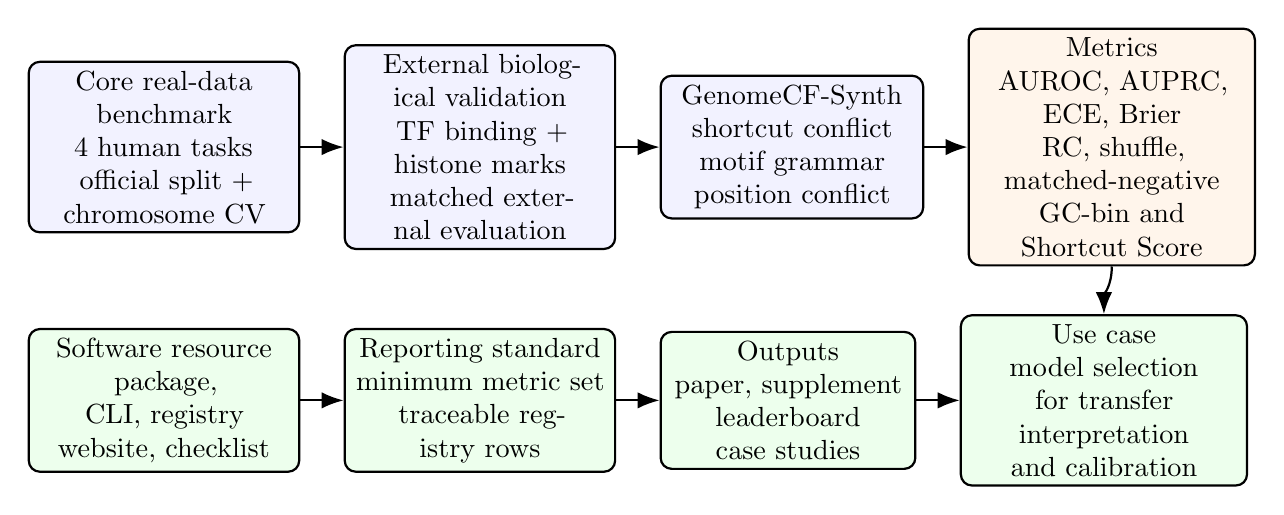
\begin{tikzpicture}[
    node distance=0.55cm and 0.55cm,
    box/.style={draw, rounded corners, thick, align=center, minimum height=0.95cm, fill=blue!5},
    metric/.style={draw, rounded corners, thick, align=center, minimum height=0.95cm, fill=orange!8},
    resource/.style={draw, rounded corners, thick, align=center, minimum height=0.95cm, fill=green!7},
    arrow/.style={-{Latex[length=2.8mm]}, thick}
  ]
    \node[box, text width=3.2cm] (core) {Core real-data benchmark\\4 human tasks\\official split + chromosome CV};
    \node[box, right=of core, text width=3.2cm] (external) {External biological validation\\TF binding + histone marks\\matched external evaluation};
    \node[box, right=of external, text width=3.1cm] (synth) {GenomeCF-Synth\\shortcut conflict\\motif grammar\\position conflict};
    \node[metric, right=of synth, text width=3.4cm] (metrics) {Metrics\\AUROC, AUPRC, ECE, Brier\\RC, shuffle, matched-negative\\GC-bin and Shortcut Score};

    \node[resource, below=1.2cm of core, text width=3.2cm] (software) {Software resource\\package, CLI, registry\\website, checklist};
    \node[resource, right=of software, text width=3.2cm] (report) {Reporting standard\\minimum metric set\\traceable registry rows};
    \node[resource, right=of report, text width=3.0cm] (outputs) {Outputs\\paper, supplement\\leaderboard\\case studies};
    \node[resource, right=of outputs, text width=3.4cm] (use) {Use case\\model selection for transfer\\interpretation and calibration};

    \draw[arrow] (core) -- (external);
    \draw[arrow] (external) -- (synth);
    \draw[arrow] (synth) -- (metrics);
    \draw[arrow] (metrics.south) to[out=-90,in=90] (use.north);
    \draw[arrow] (software) -- (report);
    \draw[arrow] (report) -- (outputs);
    \draw[arrow] (outputs) -- (use);
  \end{tikzpicture}
  \caption{GenomeCF resource overview. GenomeCF combines counterfactual stress tests on core real-data tasks, external biological assays, GenomeCF-Synth mechanism tasks, and a software/reporting stack designed for reusable community evaluation.}
  \label{fig:overview}
\end{figure*}

\begin{table*}[t]
  \centering
  \caption{GenomeCF real-data task overview. The core tier supports the main results; screening tasks are kept separate from the main claims; external biological validation is reported in dedicated figures and supplementary tables.}
  \label{tab:tasks}
  \small
  \resizebox{\textwidth}{!}{\begin{tabular}{p{3.35cm}p{0.85cm}p{1.35cm}p{2.0cm}p{2.15cm}p{0.95cm}p{0.9cm}p{2.8cm}}
\toprule
Task & Species & Length & Full train/test & Eval train/val/test & P:N & Chr. meta & Coverage \\
\midrule
\multicolumn{8}{l}{\textbf{Core tasks}} \\
Promoters\\ \scriptsize\texttt{human\_nontata\_promoters} & Human & Fixed (251) & 27,097 / 9,034 & 10,000 / 2,000 / 9,034 & 4915:4119 & Yes & \shortstack[l]{Diag., 6-mer, CNNs,\\DNABERT-2, Caduceus} \\
Enhancers (Cohn)\\ \scriptsize\texttt{human\_enhancers\_cohn} & Human & Fixed (500) & 20,843 / 6,948 & 10,000 / 2,000 / 6,948 & 3474:3474 & Yes & \shortstack[l]{Diag., 6-mer, CNNs,\\DNABERT-2, Caduceus} \\
Enhancers (Ensembl)\\ \scriptsize\texttt{human\_enhancers\_ensembl} & Human & Variable (9-488) & 123,872 / 30,970 & 10,000 / 2,000 / 30,970 & 15485:15485 & Yes & \shortstack[l]{Diag., 6-mer, CNNs,\\DNABERT-2, Caduceus} \\
Open chromatin\\ \scriptsize\texttt{human\_ocr\_ensembl} & Human & Variable (112-591) & 139,804 / 34,952 & 10,000 / 2,000 / 34,952 & 17476:17476 & Yes & \shortstack[l]{Diag., 6-mer, CNNs,\\DNABERT-2, Caduceus} \\
\multicolumn{8}{l}{\textbf{Extended screening tasks}} \\
Mouse enhancers\\ \scriptsize\texttt{dummy\_mouse\_enhancers\_ensembl} & Mouse & Variable (538-4549) & 968 / 242 & 194 / 774 / 242 & 121:121 & No & 6-mer \\
Fly enhancers\\ \scriptsize\texttt{drosophila\_enhancers\_stark} & Fly & Variable (1607-2921) & 5,184 / 1,730 & 3,184 / 2,000 / 1,730 & 865:865 & No & 6-mer \\
\bottomrule
\end{tabular}
}
\end{table*}

\subsection{Held-out AUROC does not predict counterfactual biological consistency}
The central benchmark result remains unchanged after expanding the evaluation protocol: average held-out AUROC and counterfactual biological consistency are not interchangeable quantities. Table~\ref{tab:main} shows the official core matrix. On promoters, 6-mer logistic regression reaches AUROC 0.898 yet shows reverse-complement instability 0.263, whereas the RC-aug CNN reduces that instability to 0.017. On \texttt{human\_enhancers\_cohn}, DNABERT-2 reaches AUROC 0.830 but still shows a negative mononucleotide-shuffle drop of -0.049, indicating that confidence is retained or even increased after the local sequence order is destroyed. Caduceus-Ph improves strand consistency on the focal tasks, with reverse-complement instability 0.040 on promoters and 0.030 on \texttt{human\_enhancers\_cohn}, but does not dominate DNABERT-2 on AUROC.

Figure~\ref{fig:tradeoff} makes the same point graphically. Models cluster differently depending on whether one reads AUROC, reverse-complement instability, mononucleotide behavior or ECE. The RC-aug CNN and Caduceus-Ph are consistently better on strand consistency than the 6-mer baseline and DNABERT-2, while DNABERT-2 remains strongest on average AUROC across the focal tasks. GenomeCF is designed exactly for these cases: the benchmark exposes reliability axes that standard held-out ranking collapses into a single number.

\begin{table*}[t]
  \centering
  \caption{Core official-split GenomeCF matrix. Higher AUROC is better; lower ECE, Brier, reverse-complement instability and flip rate are better. Positive mononucleotide and dinucleotide drops indicate that confidence decreases after the perturbation.}
  \label{tab:main}
  \small
  \resizebox{\textwidth}{!}{\begin{tabular}{p{3.0cm}p{2.2cm}rrrrrrr}
\toprule
Task & Model & AUROC & ECE & Brier & RC $\Delta$ & RC flip & Mono drop & Dinuc drop \\
\midrule
\shortstack[l]{Promoters} & \shortstack[l]{6-mer logistic\\regression} & 0.898 & 0.110 & 0.133 & 0.263 & 0.268 & -0.003 & 0.058 \\
\shortstack[l]{Promoters} & \shortstack[l]{CNN} & 0.843 & 0.023 & 0.152 & 0.044 & 0.062 & -0.002 & 0.046 \\
\shortstack[l]{Promoters} & \shortstack[l]{RC-aug CNN} & 0.864 & 0.044 & 0.144 & 0.017 & 0.019 & -0.035 & 0.038 \\
\shortstack[l]{Promoters} & \shortstack[l]{DNABERT-2} & 0.888 & 0.042 & 0.128 & 0.078 & 0.073 & -0.054 & 0.004 \\
\shortstack[l]{Promoters} & \shortstack[l]{Caduceus-Ph} & 0.853 & 0.024 & 0.154 & 0.040 & 0.035 & -0.060 & 0.002 \\
\shortstack[l]{Enhancers\\(Cohn)} & \shortstack[l]{6-mer logistic\\regression} & 0.700 & 0.286 & 0.309 & 0.371 & 0.378 & -0.080 & 0.138 \\
\shortstack[l]{Enhancers\\(Cohn)} & \shortstack[l]{CNN} & 0.754 & 0.079 & 0.209 & 0.019 & 0.036 & 0.008 & 0.014 \\
\shortstack[l]{Enhancers\\(Cohn)} & \shortstack[l]{RC-aug CNN} & 0.765 & 0.071 & 0.203 & 0.014 & 0.031 & 0.003 & 0.017 \\
\shortstack[l]{Enhancers\\(Cohn)} & \shortstack[l]{DNABERT-2} & 0.830 & 0.025 & 0.168 & 0.059 & 0.097 & -0.049 & 0.023 \\
\shortstack[l]{Enhancers\\(Cohn)} & \shortstack[l]{Caduceus-Ph} & 0.773 & 0.034 & 0.195 & 0.030 & 0.053 & -0.103 & -0.021 \\
\shortstack[l]{Enhancers\\(Ensembl)} & \shortstack[l]{6-mer logistic\\regression} & 0.736 & 0.246 & 0.273 & 0.344 & 0.356 & 0.203 & 0.216 \\
\shortstack[l]{Enhancers\\(Ensembl)} & \shortstack[l]{CNN} & 0.839 & 0.080 & 0.172 & 0.089 & 0.133 & 0.178 & 0.065 \\
\shortstack[l]{Enhancers\\(Ensembl)} & \shortstack[l]{RC-aug CNN} & 0.884 & 0.040 & 0.139 & 0.069 & 0.070 & 0.320 & 0.127 \\
\shortstack[l]{Enhancers\\(Ensembl)} & \shortstack[l]{DNABERT-2} & 0.775 & 0.027 & 0.194 & 0.096 & 0.146 & 0.043 & 0.009 \\
\shortstack[l]{Enhancers\\(Ensembl)} & \shortstack[l]{Caduceus-Ph} & 0.718 & 0.043 & 0.217 & 0.046 & 0.138 & -0.032 & -0.009 \\
\shortstack[l]{Open\\chromatin} & \shortstack[l]{6-mer logistic\\regression} & 0.650 & 0.296 & 0.331 & 0.380 & 0.394 & 0.227 & 0.062 \\
\shortstack[l]{Open\\chromatin} & \shortstack[l]{CNN} & 0.640 & 0.063 & 0.243 & 0.013 & 0.057 & 0.003 & -0.010 \\
\shortstack[l]{Open\\chromatin} & \shortstack[l]{RC-aug CNN} & 0.704 & 0.052 & 0.222 & 0.056 & 0.156 & 0.061 & 0.008 \\
\shortstack[l]{Open\\chromatin} & \shortstack[l]{DNABERT-2} & 0.682 & 0.022 & 0.225 & 0.090 & 0.222 & 0.086 & -0.033 \\
\shortstack[l]{Open\\chromatin} & \shortstack[l]{Caduceus-Ph} & 0.623 & 0.057 & 0.242 & 0.023 & 0.160 & -0.017 & -0.018 \\
\bottomrule
\end{tabular}
}
\end{table*}

\begin{figure*}[t]
  \centering
  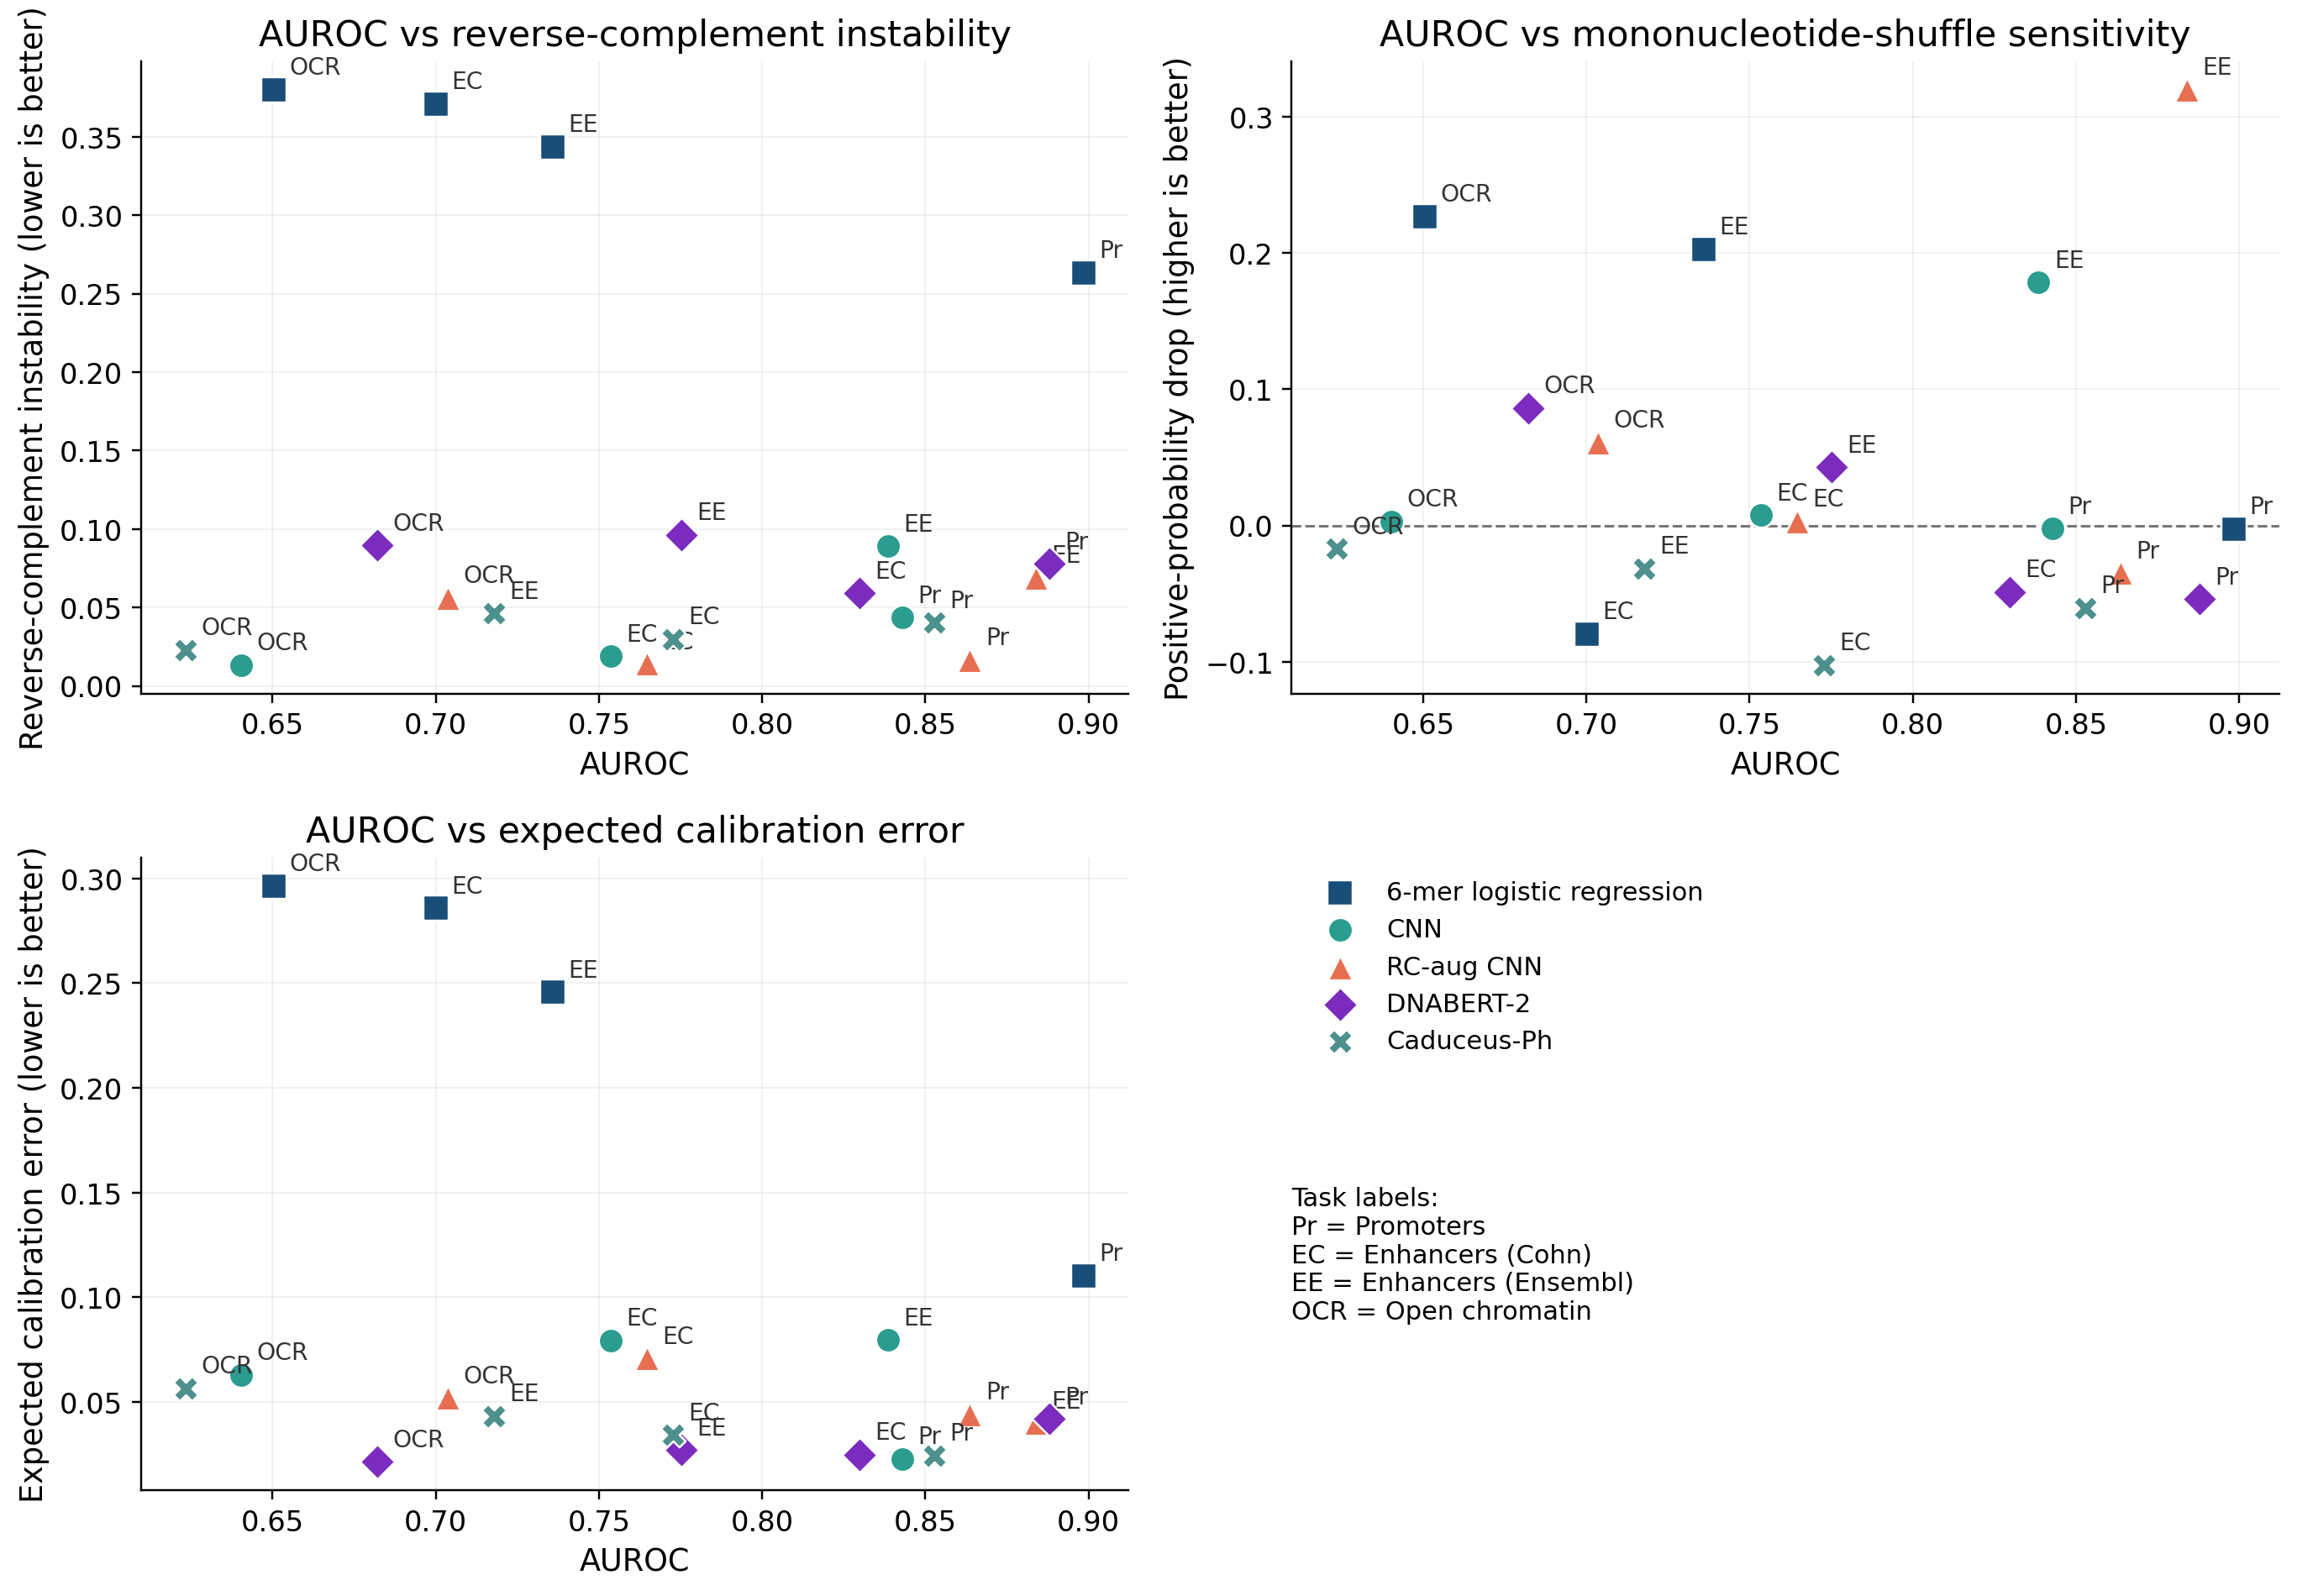
\includegraphics[width=\textwidth]{../figures/genomecf_tradeoff_publication.png}
  \caption{Held-out AUROC versus three GenomeCF axes on the four core human tasks. High AUROC does not guarantee low reverse-complement instability, biologically sensible shuffle behavior or good calibration. Task labels are Pr = Promoters, EC = Enhancers (Cohn), EE = Enhancers (Ensembl), and OCR = Open chromatin.}
  \label{fig:tradeoff}
\end{figure*}

\subsection{Foundation models differ in strand consistency, calibration and adaptation behavior}
The two completed main-paper foundation models, DNABERT-2 and Caduceus-Ph, differ along several axes that matter for biological use. DNABERT-2 is stronger on AUROC across most core tasks, whereas Caduceus-Ph consistently reduces reverse-complement instability on the focal tasks. Figure~\ref{fig:foundation} summarizes these differences and adds completed foundation-model adaptation results on the focal tasks.

The adaptation results are particularly important for practical use. We did not rely only on temperature scaling. GenomeCF now includes matched-negative-trained frozen heads for DNABERT-2 and Caduceus-Ph. On promoters, DNABERT-2 changes from official AUROC 0.913 and matched-negative AUROC 0.897 to 0.908 and 0.910 after matched-negative head training. Caduceus-Ph changes from 0.853 and 0.793 to 0.862 and 0.811. On \texttt{human\_enhancers\_cohn}, Caduceus-Ph changes from 0.773 and 0.693 to 0.777 and 0.711. These are useful practical tradeoffs rather than cosmetic additions to the benchmark: GenomeCF can show when an adaptation improves robustness to confounder-controlled evaluation even if it does not maximize the standard held-out score.

\begin{figure*}[t]
  \centering
  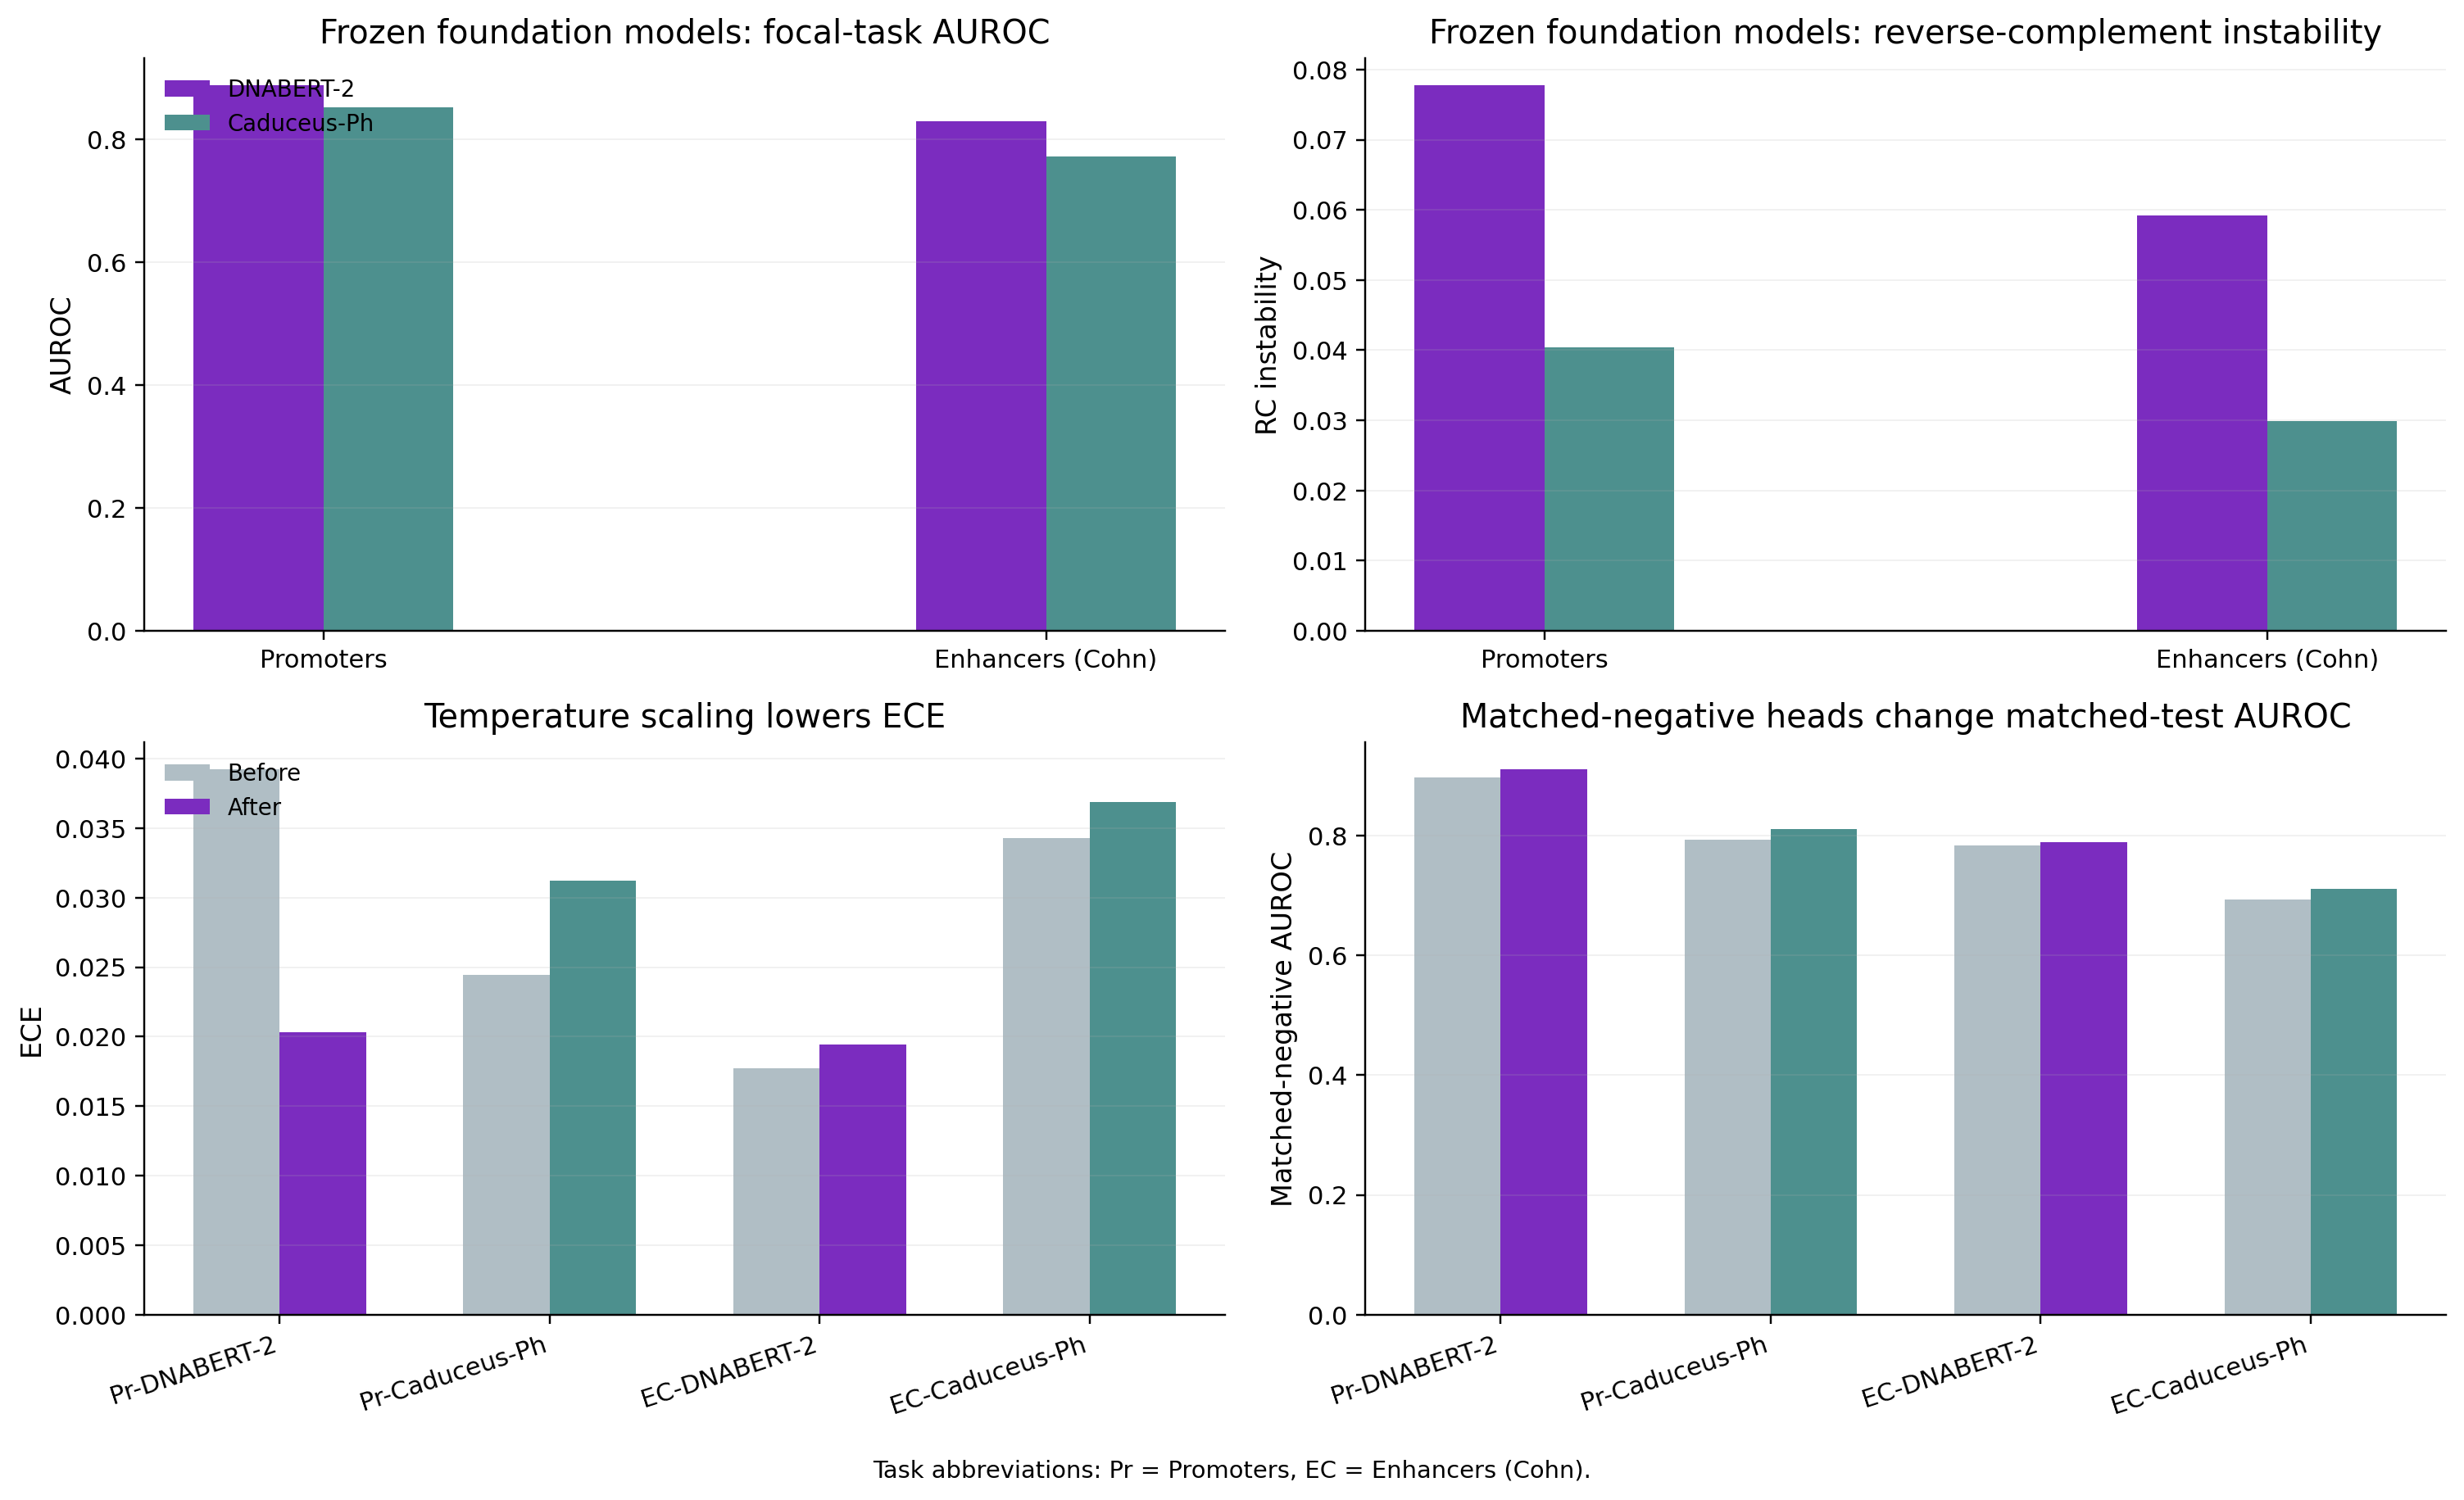
\includegraphics[width=\textwidth]{../figures/genomecf_foundation_comparison.png}
  \caption{Foundation-model comparison on the focal tasks. Top: frozen DNABERT-2 and Caduceus-Ph official AUROC and reverse-complement instability. Bottom: completed interventions on the same models. Temperature scaling improves calibration, whereas matched-negative-trained heads alter matched-test AUROC and sometimes trade off official performance for confounder-controlled robustness.}
  \label{fig:foundation}
\end{figure*}

\subsection{Chromosome-grouped cross-validation reveals split-dependent ranking shifts}
Five-fold chromosome-grouped cross-validation remains an important stress test even after external validation is added. Table~\ref{tab:cvmain} shows that the official split can overestimate performance for the classical baseline and some CNN settings, while the focal DNABERT-2 rows and all completed Caduceus-Ph rows remain comparatively stable. For example, the promoter 6-mer baseline falls from official AUROC 0.898 to mean chromosome-CV AUROC 0.834, whereas DNABERT-2 falls from 0.888 to 0.897 mean on the smaller focal CV reruns and Caduceus-Ph reaches 0.859 mean with lower strand sensitivity than the classical baseline.

These stronger splits matter because counterfactual reliability is not only about synthetic perturbations. Split robustness directly tests whether a model is carrying benchmark-specific artifacts across genomic regions. GenomeCF therefore treats chromosome-grouped cross-validation as part of the minimum reporting standard rather than an optional appendix check.

\begin{table*}[t]
  \centering
  \caption{Five-fold chromosome-grouped cross-validation on the core human tasks. Completed focal DNABERT-2 rows and completed Caduceus-Ph rows are shown alongside the lightweight baselines.}
  \label{tab:cvmain}
  \small
  \resizebox{\textwidth}{!}{\input{../results/publication/table3_cv_summary.tex}}
\end{table*}

\begin{figure*}[t]
  \centering
  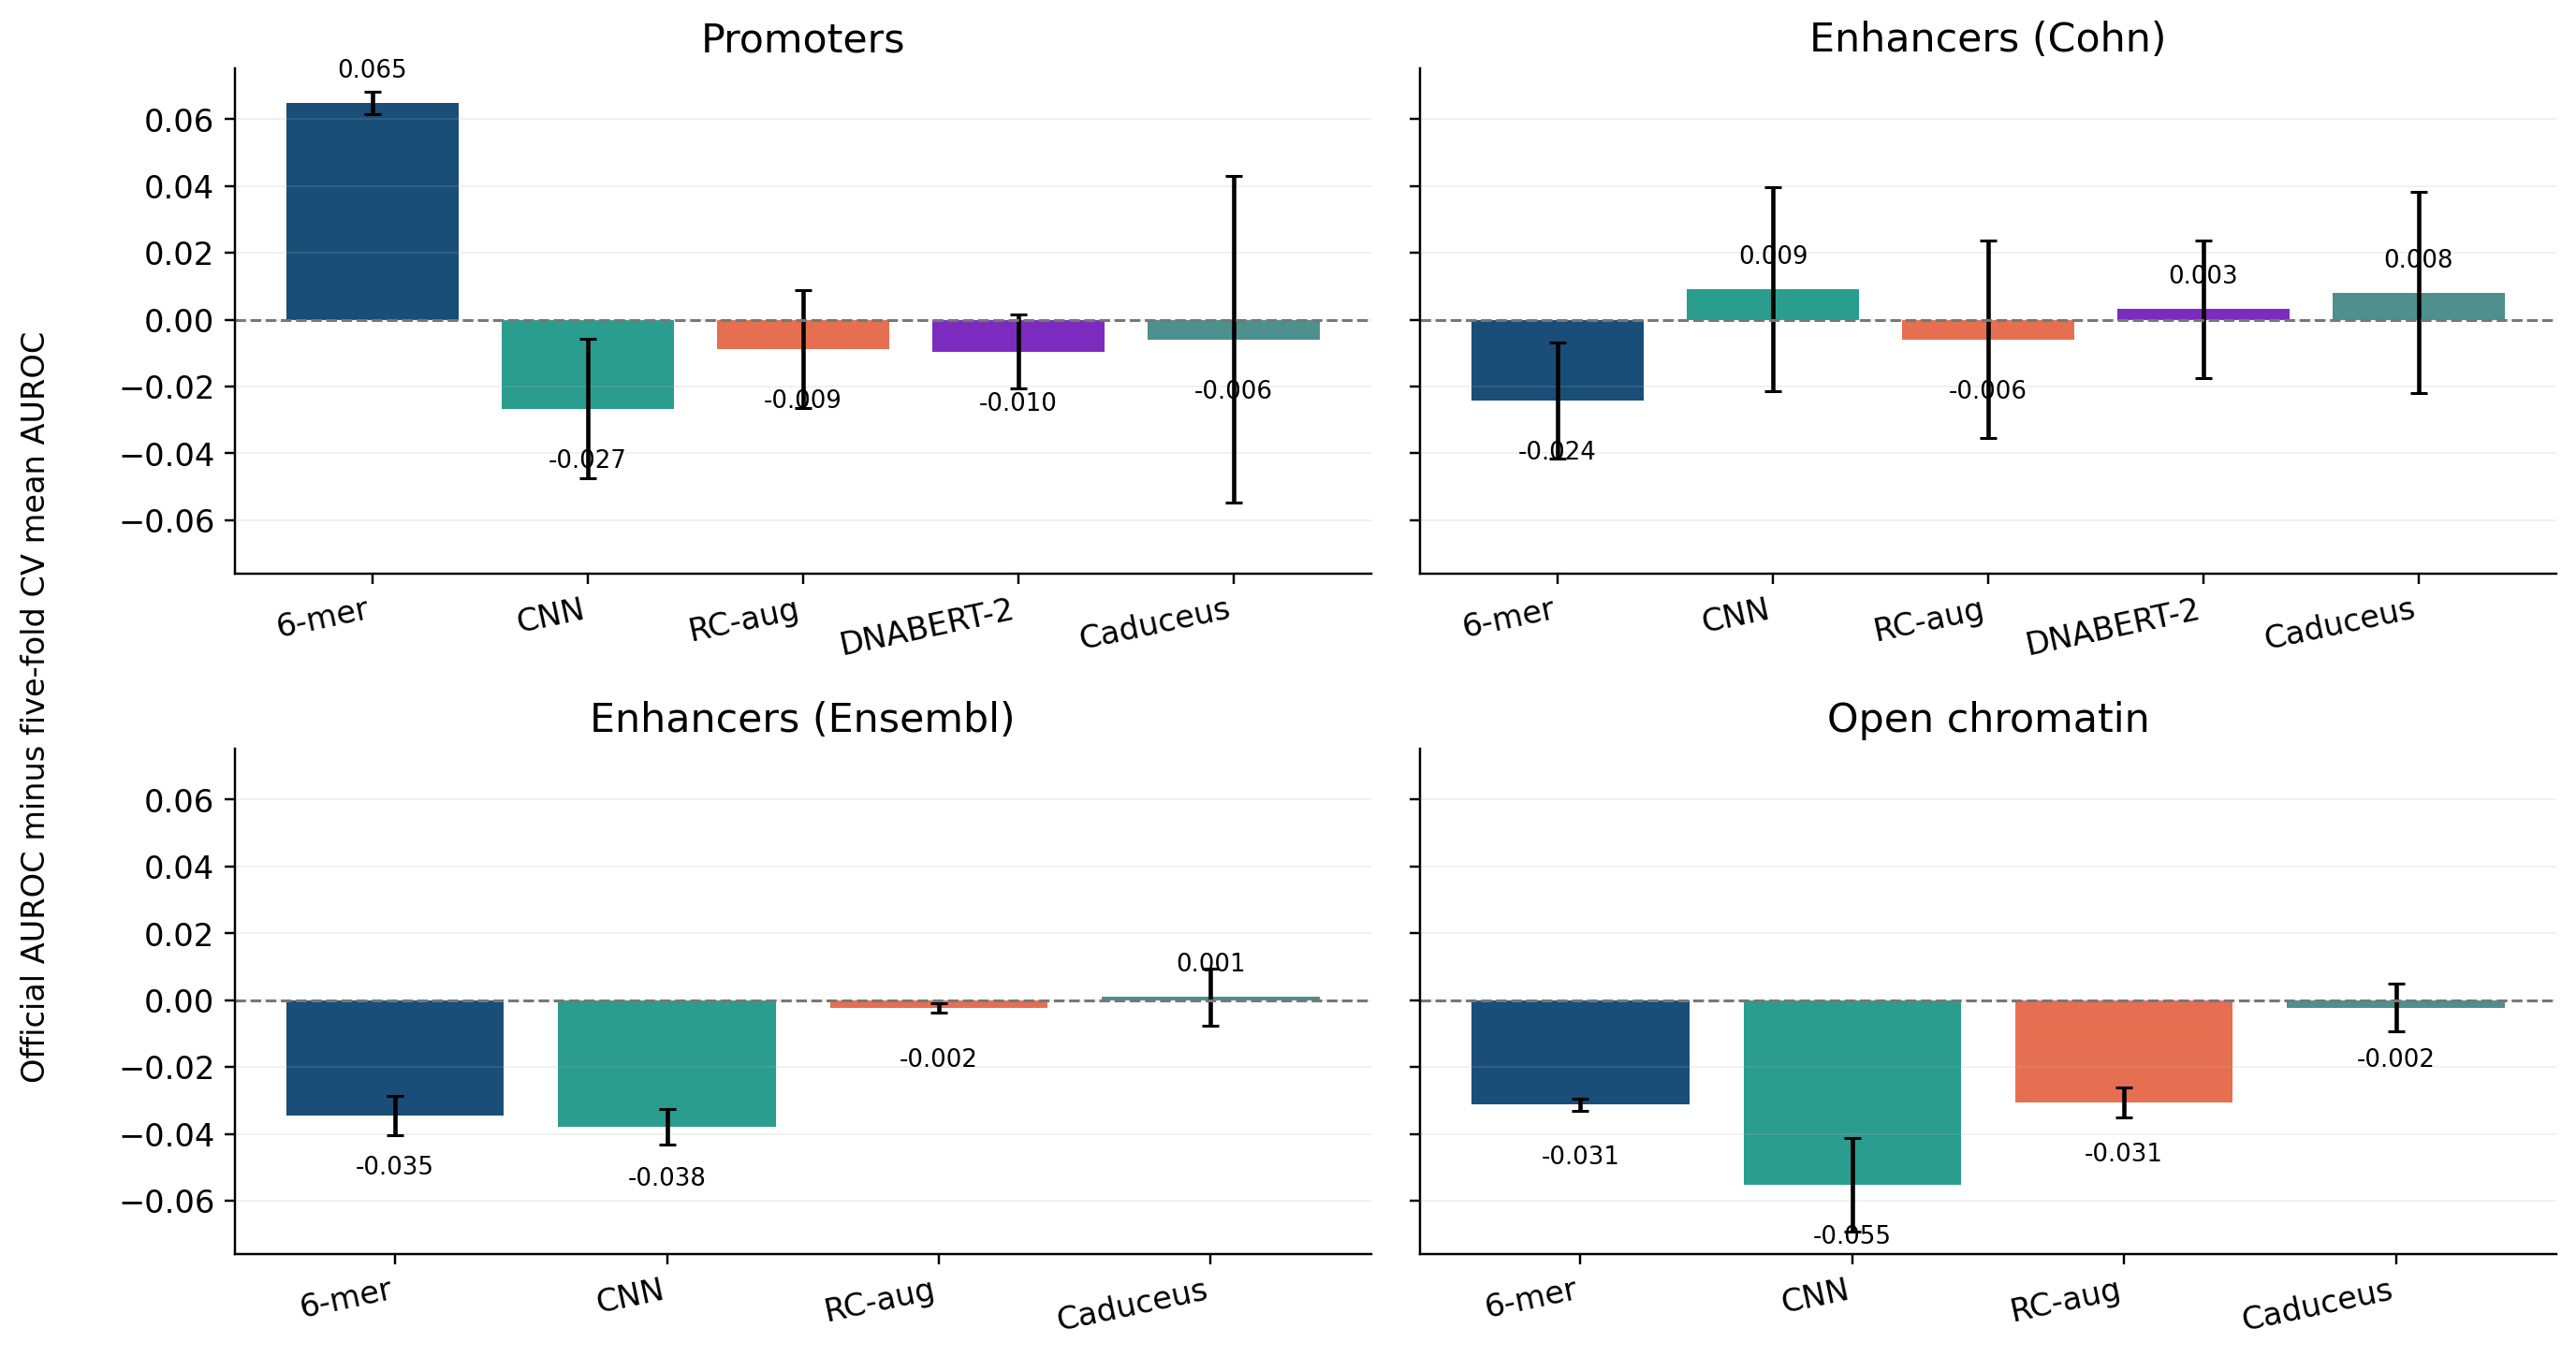
\includegraphics[width=\textwidth]{../figures/genomecf_generalization_gap.png}
  \caption{Official AUROC minus five-fold chromosome-CV mean AUROC. Error bars denote fold-to-fold standard deviation. Larger positive values indicate that the official split overestimates performance relative to chromosome-grouped evaluation.}
  \label{fig:cv}
\end{figure*}

\subsection{Matched-negative and GC-bin analyses reveal composition-dependent failure modes}
GenomeCF adds two complementary confounder-control views: matched-negative evaluation and composition-stratified robustness. The matched-negative summary in Table~\ref{tab:matched} shows that easy background structure carries real predictive signal, but not enough to explain performance on its own. Promoter GC-only AUROC falls from 0.796 to 0.712 under matched negatives. Yet the better sequence models remain substantially above chance: DNABERT-2 changes from 0.913 to 0.897, whereas Caduceus-Ph changes from 0.853 to 0.793. On \texttt{human\_enhancers\_cohn}, DNABERT-2 changes from 0.832 to 0.783 and Caduceus-Ph from 0.773 to 0.693. These are meaningful drops, but they do not erase predictive signal.

Table~\ref{tab:mitigation} shows that interventions address different failure modes. Temperature scaling reduces ECE without changing AUROC much, for example lowering promoter RC-aug CNN ECE from 0.061 to 0.030. GC-balanced training changes both calibration and perturbation behavior, but in a task-dependent way. Matched-negative retraining is stronger as a mitigation for the RC-aug CNN than for the plain CNN on promoters: the RC-aug model changes from matched-negative AUROC 0.874 to 0.893, whereas the plain CNN changes from 0.873 to 0.854. GenomeCF therefore supports practical intervention choice rather than only diagnosis.

Figure~\ref{fig:gcbin} adds a worst-group robustness view. On promoters, DNABERT-2 reaches overall AUROC 0.888 on the benchmark budget, yet its worst-GC-bin AUROC falls to 0.718 with a GC-bin gap of 0.262. Caduceus-Ph reaches lower average AUROC but also lower worst-group AUROC, 0.624. Across the enhancer tasks the ranking changes again. GenomeCF thus evaluates not only average AUROC but also whether performance collapses in specific composition strata.

\begin{table*}[t]
  \centering
  \caption{Matched-negative evaluation on the three focal real tasks. Completed rows are shown for GC-only, 6-mer logistic regression, CNN, RC-aug CNN, DNABERT-2 and Caduceus-Ph.}
  \label{tab:matched}
  \small
  \resizebox{\textwidth}{!}{\begin{tabular}{p{2.15cm}p{2.0cm}rrrrrr}
\toprule
Task & Model & Orig. AUROC & Matched AUROC & Orig. GC-only & Matched GC-only & Orig. mono & Matched mono \\
\midrule
\shortstack[l]{Promoters} & \shortstack[l]{GC-only logistic\\regression} & 0.796 & 0.712 & 0.796 & 0.712 & 0.000 & 0.000 \\
\shortstack[l]{Promoters} & \shortstack[l]{6-mer logistic\\regression} & 0.916 & 0.911 & 0.796 & 0.712 & -0.013 & -0.008 \\
\shortstack[l]{Promoters} & \shortstack[l]{CNN} & 0.891 & 0.873 & 0.796 & 0.712 & -0.034 & -0.059 \\
\shortstack[l]{Promoters} & \shortstack[l]{RC-aug CNN} & 0.901 & 0.874 & 0.796 & 0.712 & -0.066 & -0.068 \\
\shortstack[l]{Promoters} & \shortstack[l]{DNABERT-2} & 0.913 & 0.897 & 0.796 & 0.712 & -0.037 & -0.039 \\
\shortstack[l]{Promoters} & \shortstack[l]{Caduceus-Ph} & 0.853 & 0.793 & 0.796 & 0.712 & -0.060 & -0.061 \\
\shortstack[l]{Enhancers\\(Cohn)} & \shortstack[l]{GC-only logistic\\regression} & 0.734 & 0.639 & 0.734 & 0.639 & 0.000 & 0.000 \\
\shortstack[l]{Enhancers\\(Cohn)} & \shortstack[l]{6-mer logistic\\regression} & 0.720 & 0.684 & 0.734 & 0.639 & -0.099 & -0.105 \\
\shortstack[l]{Enhancers\\(Cohn)} & \shortstack[l]{CNN} & 0.750 & 0.673 & 0.734 & 0.639 & 0.025 & -0.006 \\
\shortstack[l]{Enhancers\\(Cohn)} & \shortstack[l]{RC-aug CNN} & 0.756 & 0.696 & 0.734 & 0.639 & -0.020 & 0.016 \\
\shortstack[l]{Enhancers\\(Cohn)} & \shortstack[l]{DNABERT-2} & 0.832 & 0.783 & 0.734 & 0.639 & -0.077 & -0.041 \\
\shortstack[l]{Enhancers\\(Cohn)} & \shortstack[l]{Caduceus-Ph} & 0.773 & 0.693 & 0.734 & 0.639 & -0.103 & -0.102 \\
\shortstack[l]{Enhancers\\(Ensembl)} & \shortstack[l]{GC-only logistic\\regression} & 0.662 & 0.576 & 0.662 & 0.576 & 0.000 & 0.000 \\
\shortstack[l]{Enhancers\\(Ensembl)} & \shortstack[l]{6-mer logistic\\regression} & 0.778 & 0.759 & 0.662 & 0.576 & 0.202 & 0.209 \\
\shortstack[l]{Enhancers\\(Ensembl)} & \shortstack[l]{CNN} & 0.881 & 0.864 & 0.662 & 0.576 & 0.390 & 0.376 \\
\shortstack[l]{Enhancers\\(Ensembl)} & \shortstack[l]{RC-aug CNN} & 0.887 & 0.870 & 0.662 & 0.576 & 0.365 & 0.366 \\
\shortstack[l]{Enhancers\\(Ensembl)} & \shortstack[l]{DNABERT-2} & 0.775 & 0.774 & 0.662 & 0.576 & 0.043 & 0.092 \\
\shortstack[l]{Enhancers\\(Ensembl)} & \shortstack[l]{Caduceus-Ph} & 0.718 & 0.652 & 0.662 & 0.576 & -0.032 & -0.032 \\
\bottomrule
\end{tabular}
}
\end{table*}

\begin{table*}[t]
  \centering
  \caption{Completed mitigation experiments. Temperature scaling targets calibration, GC-balanced training targets composition-sensitive training behavior, and matched-negative retraining targets background-construction bias.}
  \label{tab:mitigation}
  \small
  \resizebox{\textwidth}{!}{\begin{tabular}{p{1.8cm}p{1.7cm}p{1.9cm}rrrrrrrrrr}
\toprule
Task & Model & Intervention & AUROC before & AUROC after & ECE before & ECE after & Brier before & Brier after & Mono before & Mono after & Matched AUROC before & Matched AUROC after \\
\midrule
\shortstack[l]{Promoters} & \shortstack[l]{CNN} & \shortstack[l]{Temperature\\scaling} & 0.891 & 0.875 & 0.024 & 0.039 & 0.129 & 0.135 & -0.034 & 0.000 & 0.873 & -- \\
\shortstack[l]{Promoters} & \shortstack[l]{CNN} & \shortstack[l]{GC-balanced\\training} & 0.891 & 0.874 & 0.024 & 0.132 & 0.129 & 0.163 & -0.034 & 0.028 & 0.873 & -- \\
\shortstack[l]{Promoters} & \shortstack[l]{CNN} & \shortstack[l]{Matched-negative\\retraining} & 0.891 & 0.871 & 0.024 & 0.067 & 0.129 & 0.142 & -0.034 & -0.037 & 0.873 & 0.854 \\
\shortstack[l]{Promoters} & \shortstack[l]{RC-aug CNN} & \shortstack[l]{Temperature\\scaling} & 0.901 & 0.897 & 0.061 & 0.030 & 0.124 & 0.119 & -0.066 & -0.033 & 0.874 & -- \\
\shortstack[l]{Promoters} & \shortstack[l]{RC-aug CNN} & \shortstack[l]{GC-balanced\\training} & 0.901 & 0.901 & 0.061 & 0.040 & 0.124 & 0.117 & -0.066 & -0.052 & 0.874 & -- \\
\shortstack[l]{Promoters} & \shortstack[l]{RC-aug CNN} & \shortstack[l]{Matched-negative\\retraining} & 0.901 & 0.882 & 0.061 & 0.078 & 0.124 & 0.139 & -0.066 & -0.062 & 0.874 & 0.893 \\
\shortstack[l]{Promoters} & \shortstack[l]{DNABERT-2} & \shortstack[l]{Temperature\\scaling} & 0.913 & 0.913 & 0.039 & 0.020 & 0.111 & 0.113 & -0.037 & -0.049 & 0.897 & 0.897 \\
\shortstack[l]{Promoters} & \shortstack[l]{DNABERT-2} & \shortstack[l]{Matched-negative\\retraining} & 0.913 & 0.908 & 0.039 & 0.112 & 0.111 & 0.137 & -0.037 & -0.049 & 0.897 & 0.910 \\
\shortstack[l]{Promoters} & \shortstack[l]{Caduceus-Ph} & \shortstack[l]{Temperature\\scaling} & 0.853 & 0.853 & 0.024 & 0.031 & 0.154 & 0.155 & -0.060 & -0.068 & 0.793 & 0.793 \\
\shortstack[l]{Promoters} & \shortstack[l]{Caduceus-Ph} & \shortstack[l]{Matched-negative\\retraining} & 0.853 & 0.862 & 0.024 & 0.140 & 0.154 & 0.175 & -0.060 & -0.049 & 0.793 & 0.811 \\
\shortstack[l]{Enhancers\\(Cohn)} & \shortstack[l]{CNN} & \shortstack[l]{Temperature\\scaling} & 0.750 & 0.761 & 0.037 & 0.040 & 0.204 & 0.200 & 0.025 & 0.020 & 0.673 & -- \\
\shortstack[l]{Enhancers\\(Cohn)} & \shortstack[l]{CNN} & \shortstack[l]{GC-balanced\\training} & 0.750 & 0.752 & 0.037 & 0.120 & 0.204 & 0.219 & 0.025 & 0.001 & 0.673 & -- \\
\shortstack[l]{Enhancers\\(Cohn)} & \shortstack[l]{CNN} & \shortstack[l]{Matched-negative\\retraining} & 0.750 & 0.739 & 0.037 & 0.109 & 0.204 & 0.228 & 0.025 & -0.013 & 0.673 & 0.672 \\
\shortstack[l]{Enhancers\\(Cohn)} & \shortstack[l]{RC-aug CNN} & \shortstack[l]{Temperature\\scaling} & 0.756 & 0.765 & 0.035 & 0.020 & 0.202 & 0.198 & -0.020 & 0.020 & 0.696 & -- \\
\shortstack[l]{Enhancers\\(Cohn)} & \shortstack[l]{RC-aug CNN} & \shortstack[l]{GC-balanced\\training} & 0.756 & 0.767 & 0.035 & 0.062 & 0.202 & 0.201 & -0.020 & 0.013 & 0.696 & -- \\
\shortstack[l]{Enhancers\\(Cohn)} & \shortstack[l]{RC-aug CNN} & \shortstack[l]{Matched-negative\\retraining} & 0.756 & 0.757 & 0.035 & 0.102 & 0.202 & 0.218 & -0.020 & -0.008 & 0.696 & 0.683 \\
\shortstack[l]{Enhancers\\(Cohn)} & \shortstack[l]{DNABERT-2} & \shortstack[l]{Temperature\\scaling} & 0.832 & 0.833 & 0.018 & 0.019 & 0.167 & 0.167 & -0.077 & -0.042 & 0.783 & 0.783 \\
\shortstack[l]{Enhancers\\(Cohn)} & \shortstack[l]{DNABERT-2} & \shortstack[l]{Matched-negative\\retraining} & 0.832 & 0.820 & 0.018 & 0.073 & 0.167 & 0.180 & -0.077 & -0.110 & 0.783 & 0.789 \\
\shortstack[l]{Enhancers\\(Cohn)} & \shortstack[l]{Caduceus-Ph} & \shortstack[l]{Temperature\\scaling} & 0.773 & 0.774 & 0.034 & 0.037 & 0.195 & 0.194 & -0.103 & -0.112 & 0.693 & 0.696 \\
\shortstack[l]{Enhancers\\(Cohn)} & \shortstack[l]{Caduceus-Ph} & \shortstack[l]{Matched-negative\\retraining} & 0.773 & 0.777 & 0.034 & 0.089 & 0.195 & 0.206 & -0.103 & -0.105 & 0.693 & 0.711 \\
\shortstack[l]{Enhancers\\(Ensembl)} & \shortstack[l]{CNN} & \shortstack[l]{GC-balanced\\training} & 0.881 & 0.873 & 0.053 & 0.092 & 0.144 & 0.157 & 0.390 & 0.375 & 0.864 & -- \\
\shortstack[l]{Enhancers\\(Ensembl)} & \shortstack[l]{CNN} & \shortstack[l]{Matched-negative\\retraining} & 0.881 & 0.859 & 0.053 & 0.148 & 0.144 & 0.179 & 0.390 & 0.254 & 0.864 & 0.849 \\
\shortstack[l]{Enhancers\\(Ensembl)} & \shortstack[l]{RC-aug CNN} & \shortstack[l]{GC-balanced\\training} & 0.887 & 0.886 & 0.034 & 0.047 & 0.138 & 0.140 & 0.365 & 0.358 & 0.870 & -- \\
\shortstack[l]{Enhancers\\(Ensembl)} & \shortstack[l]{RC-aug CNN} & \shortstack[l]{Matched-negative\\retraining} & 0.887 & 0.874 & 0.034 & 0.098 & 0.138 & 0.157 & 0.365 & 0.336 & 0.870 & 0.864 \\
\bottomrule
\end{tabular}
}
\end{table*}

\begin{figure*}[t]
  \centering
  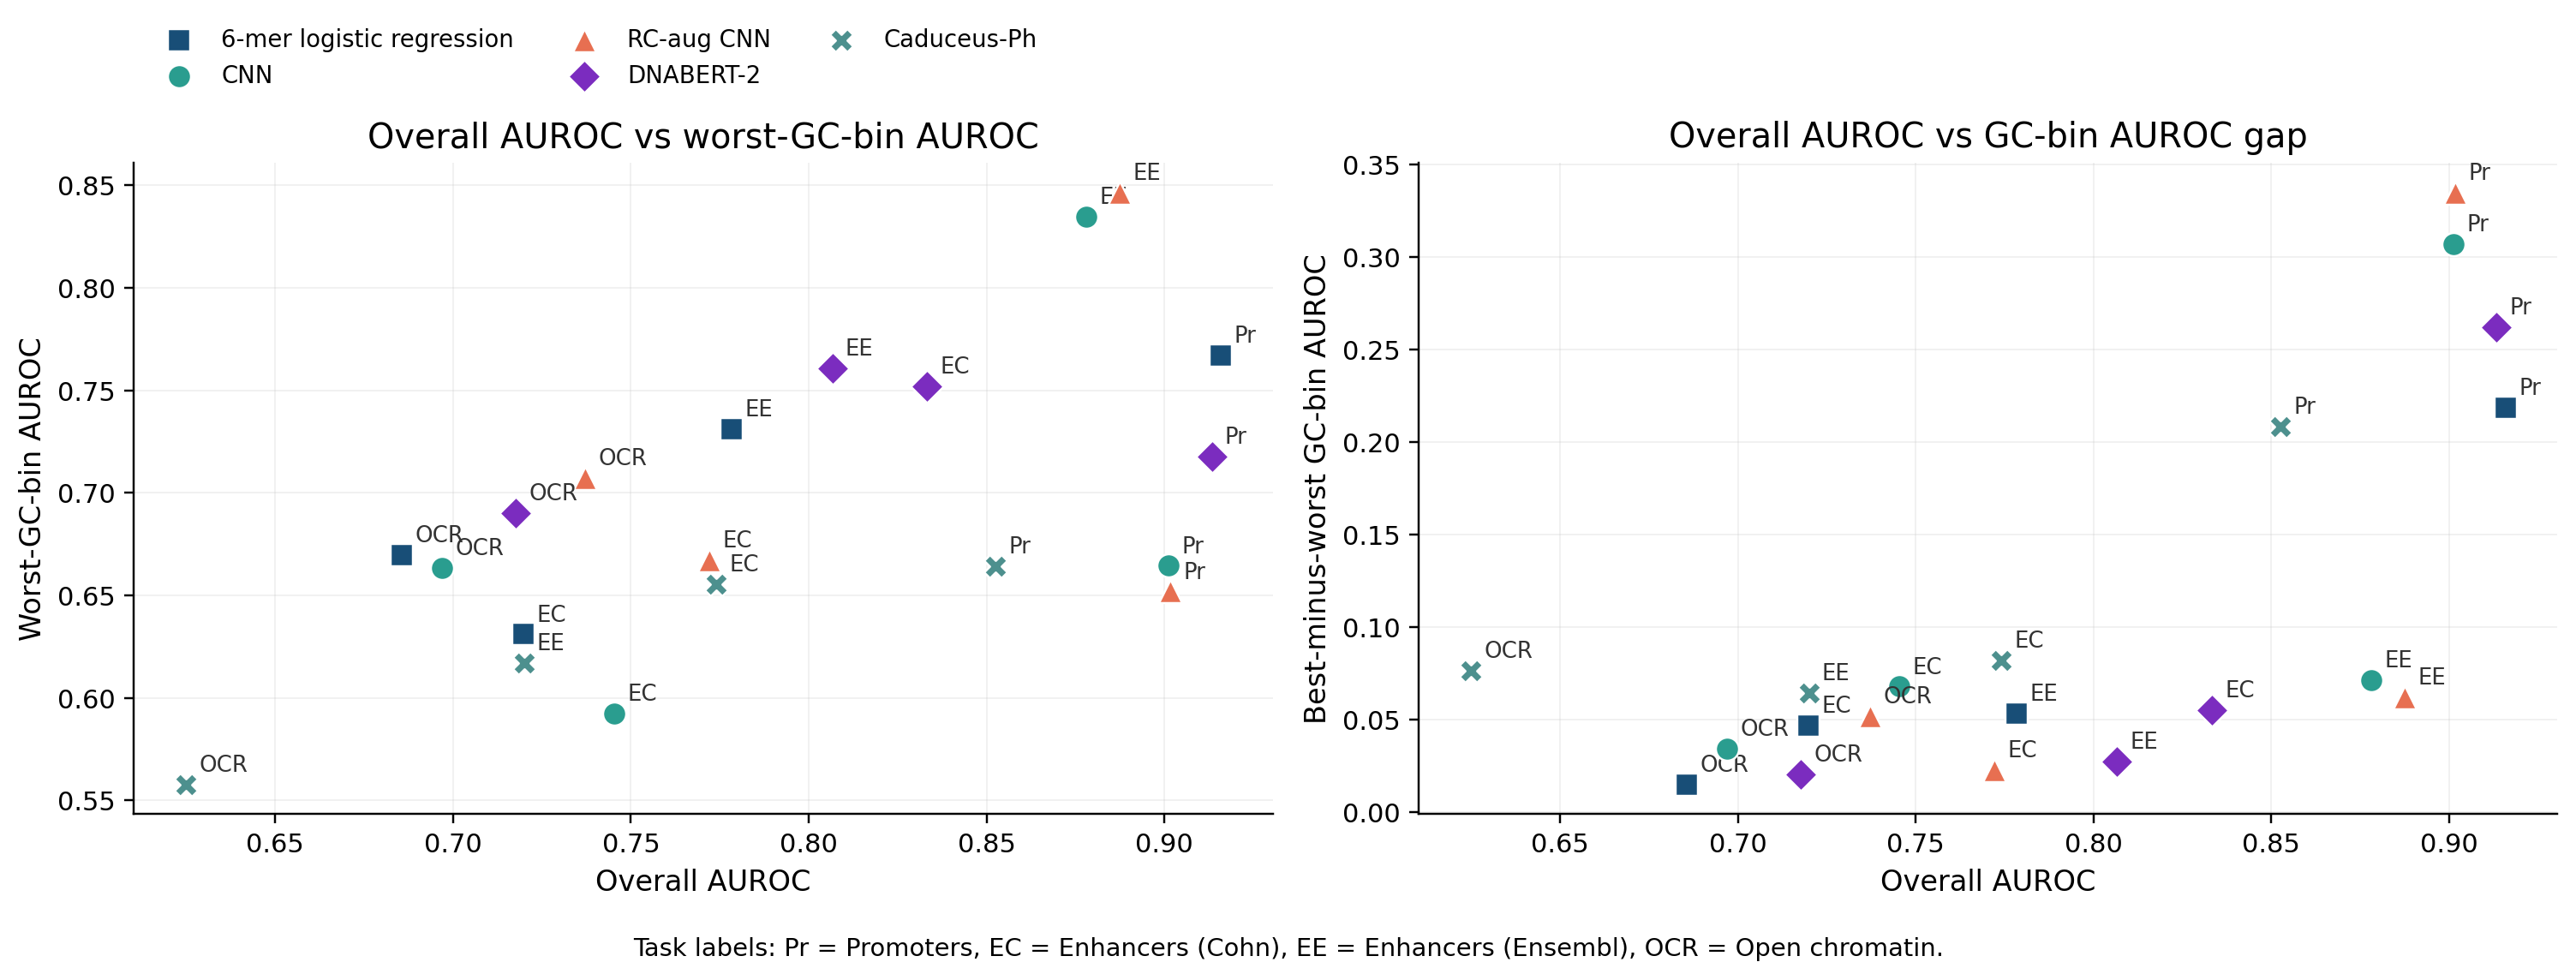
\includegraphics[width=\textwidth]{../figures/genomecf_gc_bin_robustness.png}
  \caption{GC-bin robustness on the four core human tasks. The left panel compares overall AUROC to worst-GC-bin AUROC, and the right panel shows the best-minus-worst AUROC gap across GC quantile bins. Lower gap is better.}
  \label{fig:gcbin}
\end{figure*}

\subsection{GenomeCF metrics predict external biological transfer and variant-effect reliability}
The most important Nature Methods-style result is that GenomeCF metrics retain explanatory power on external biological assays. We integrated three external assay families beyond the core benchmark: human transcription-factor binding and histone-mark classification tasks from the GUE release \citep{zhou2024dnabert2}, plus five public human regulatory MPRA variant-effect tasks curated through MaveDB and derived from the saturation-mutagenesis study of disease-associated regulatory elements by \citet{kircher2019regulatory}. These additions extend GenomeCF from sequence classification into experimentally measured regulatory variant interpretation.

Figure~\ref{fig:external} and Supplementary Tables~S11--S13 summarize the expanded external analysis. Across the two TF-binding tasks, DNABERT-2 achieves the strongest mean official AUROC at 0.884, while Caduceus-Ph is lower at 0.780 but remains more strand-consistent on the core benchmark. Across the two histone-mark tasks, DNABERT-2 again leads by AUROC at 0.702. The five MPRA tasks tell a different story: the 6-mer baseline averages AUROC 0.646, Spearman correlation 0.259 against absolute measured effect size, and top-$k$ enrichment 1.49, whereas DNABERT-2 averages AUROC 0.557, Spearman 0.090 and top-$k$ enrichment 1.34. Caduceus-Ph is now included across all five MPRA tasks under the same frozen-head protocol, but in this compact variant-effect setting it averages AUROC 0.497, AUPRC 0.359 and worst-GC-bin AUROC 0.415. GenomeCF therefore reveals that benchmark leaders are not automatically the strongest variant-effect models and that stronger strand consistency on the core benchmark does not by itself guarantee better compact MPRA reliability.

The expanded external analysis now covers 82 model-configuration-task pairs across the three assay families. Table~\ref{tab:external-predict} shows that held-out core AUROC alone explains only 6.2\% of the variance in external biological reliability under this broader analysis, whereas the compact GenomeCF Shortcut Score explains 2.3\%, and a fuller GenomeCF profile combining shortcut, calibration, matched-negative and GC-bin metrics explains 38.3\% (95\% CI 26.3--56.4\%). The full GenomeCF profile therefore improves over AUROC alone by 0.321 $R^2$ units (95\% CI 0.182--0.515). Leave-one-family-out prediction remains challenging because assay families define different biological failure modes, but the full profile still improves over AUROC alone (cross-family $R^2 = -0.109$ versus $-0.318$), and family-stratified fits are substantially stronger for the fuller GenomeCF profile than for AUROC alone. GenomeCF therefore contributes information about external biological reliability that is not recoverable from held-out benchmark AUROC alone, while also showing honestly that fully assay-agnostic extrapolation remains difficult.

\begin{figure*}[t]
  \centering
  \begin{subfigure}[t]{0.49\textwidth}
    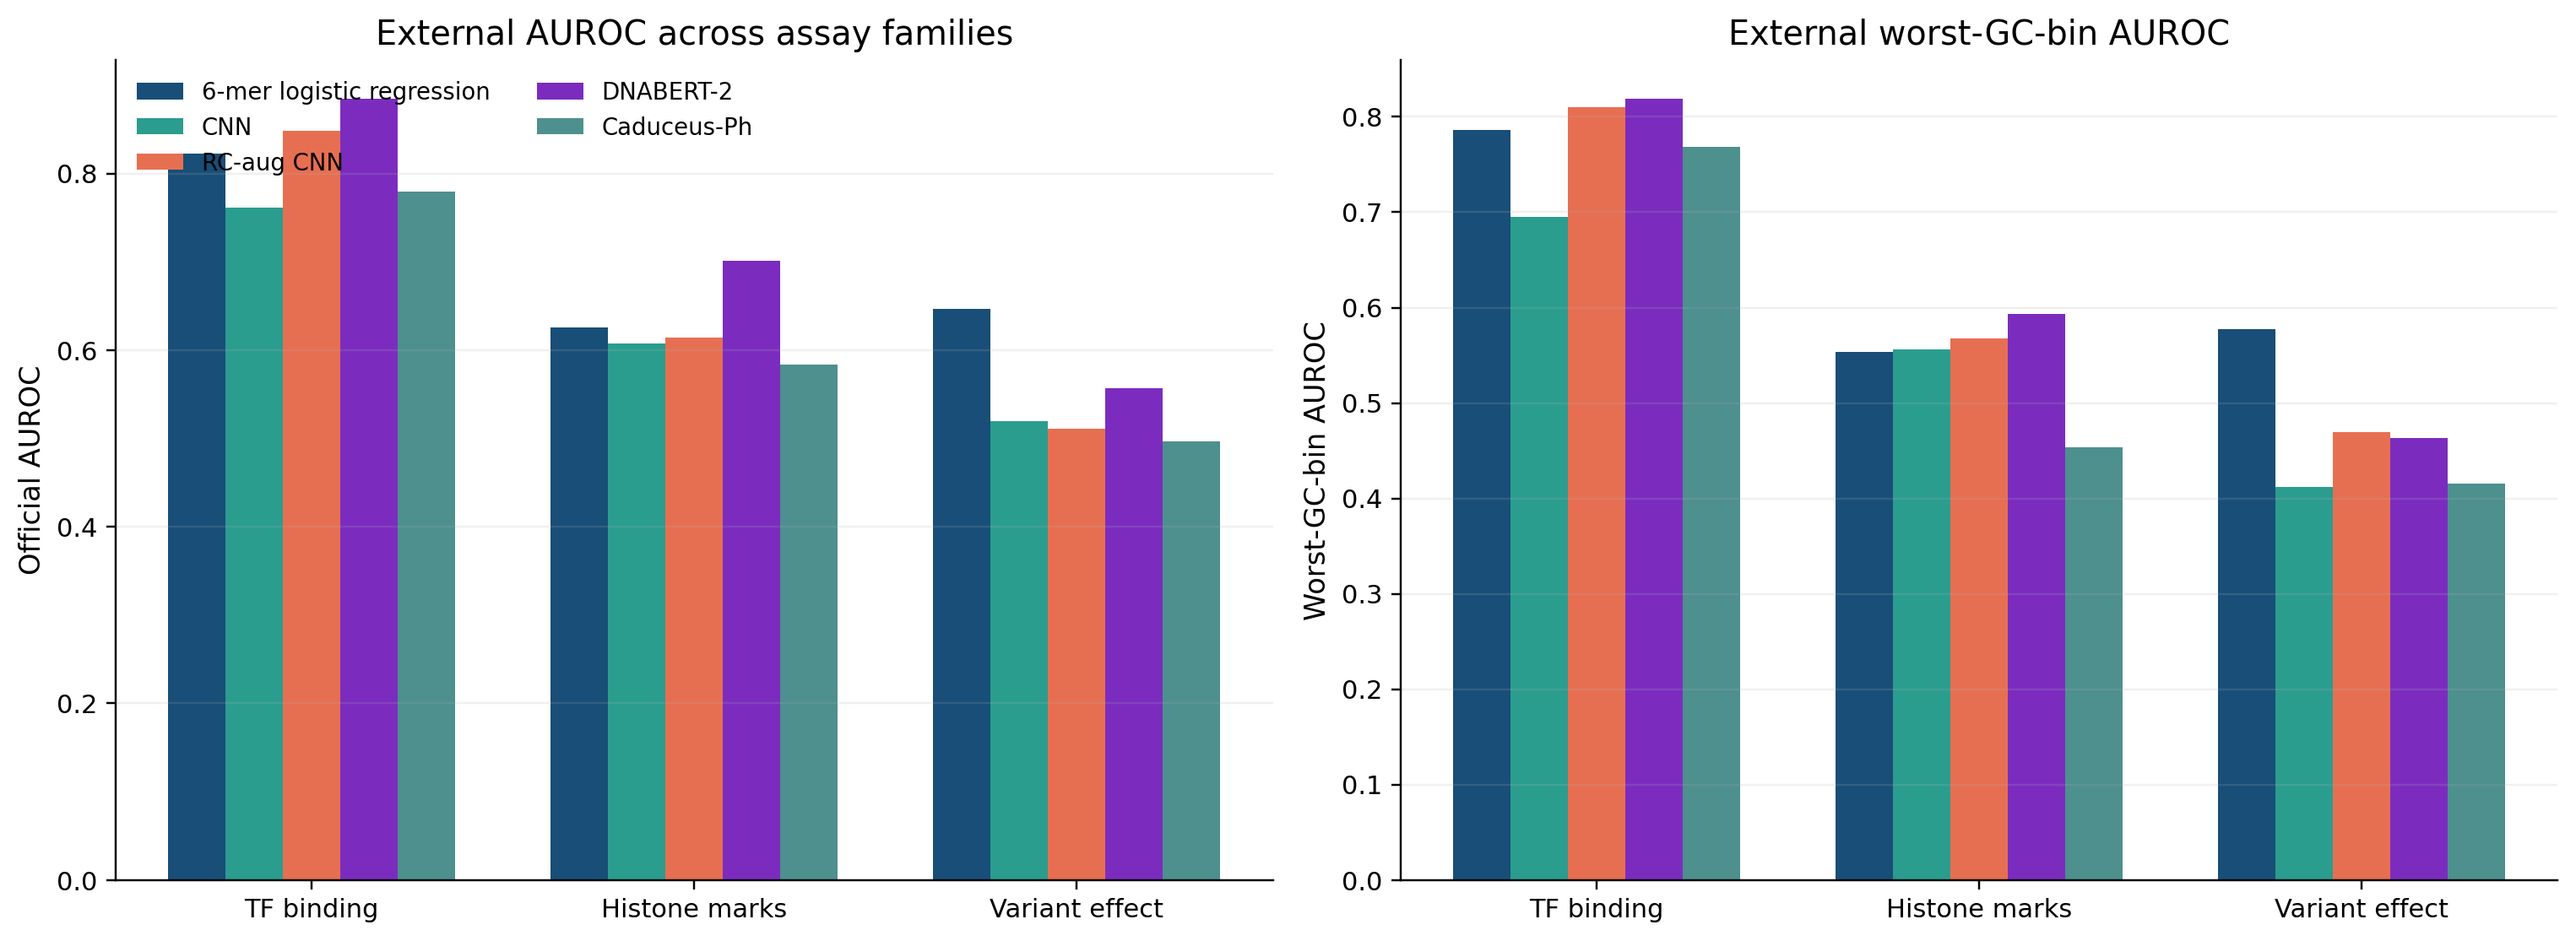
\includegraphics[width=\textwidth]{../figures/genomecf_external_validation.png}
    \caption{External assay-family performance}
  \end{subfigure}
  \hfill
  \begin{subfigure}[t]{0.49\textwidth}
    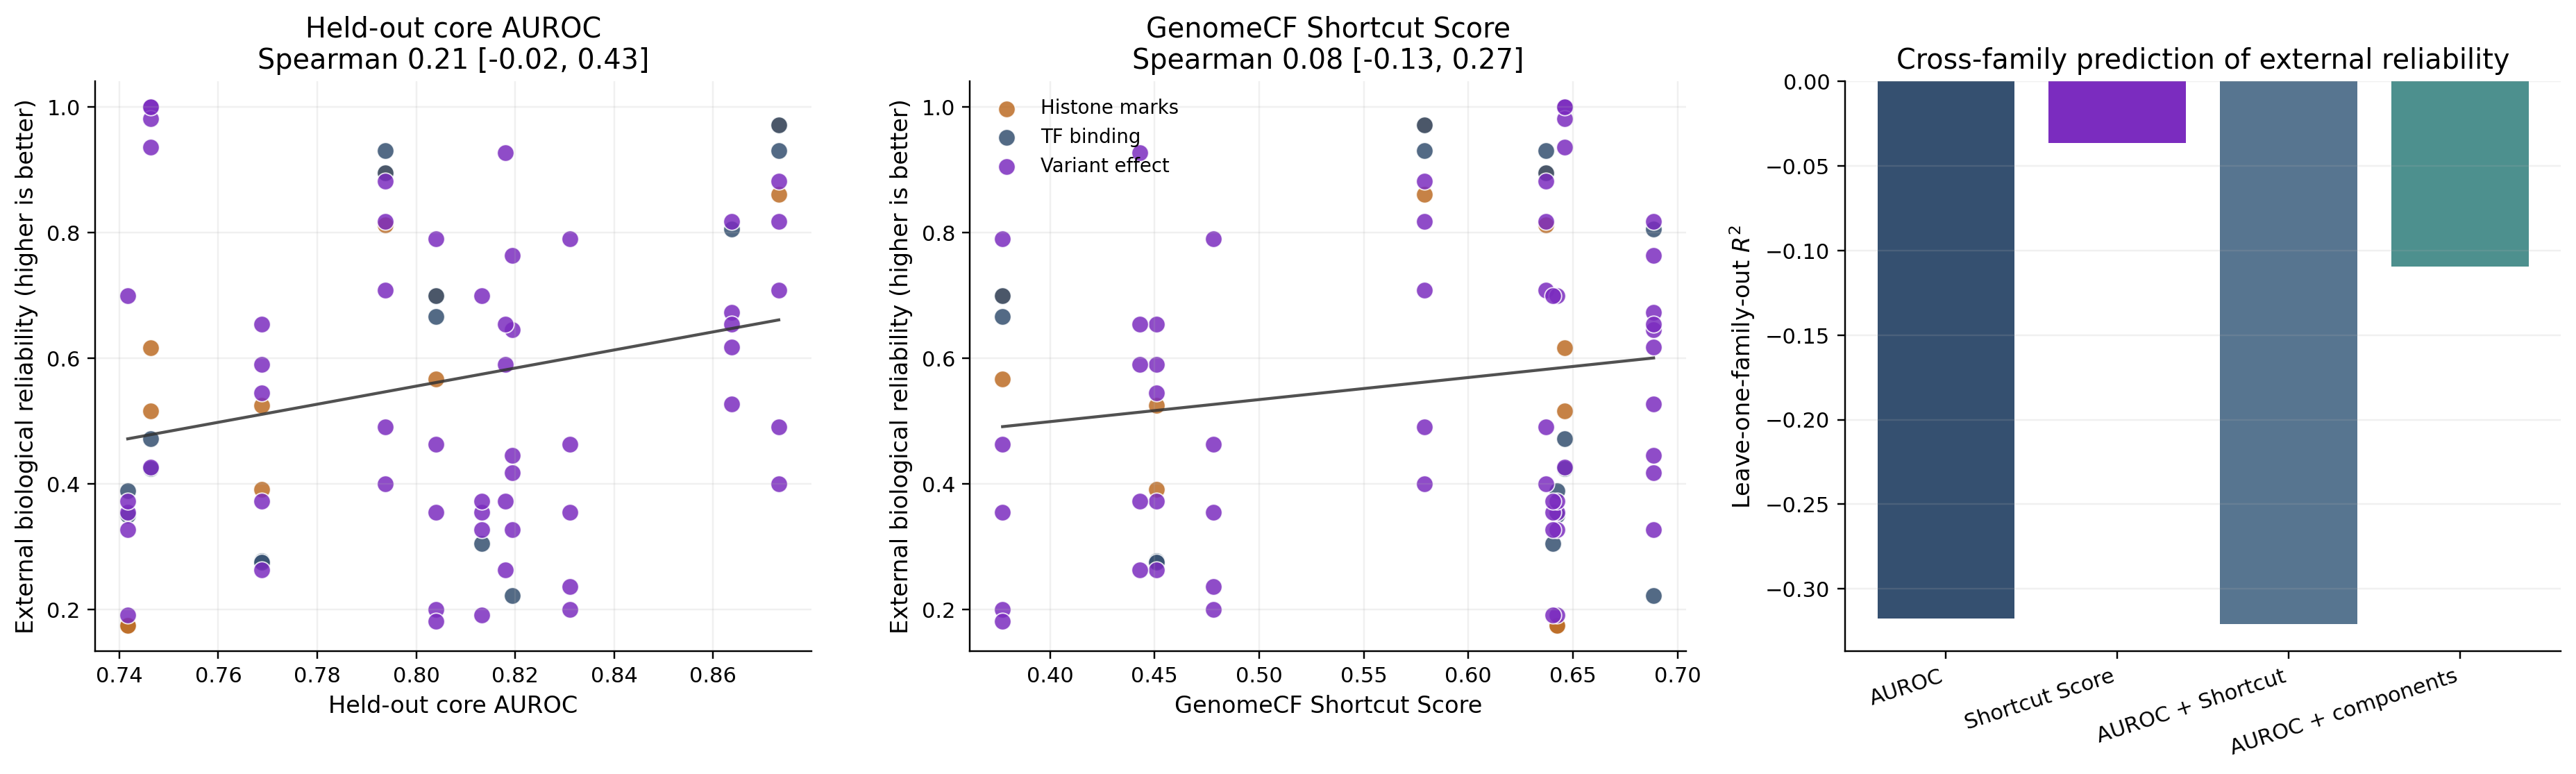
\includegraphics[width=\textwidth]{../figures/genomecf_external_prediction.png}
    \caption{GenomeCF predicts external biological reliability}
  \end{subfigure}
  \caption{External biological validation. Left, official and worst-bin assay-family results across TF-binding, histone-mark and MPRA variant-effect tasks. Right, external biological reliability is better explained by GenomeCF counterfactual metrics than by held-out core AUROC alone.}
  \label{fig:external}
\end{figure*}

\begin{table*}[t]
  \centering
  \caption{GenomeCF prediction of external biological reliability. The table reports the main cross-task correlation, regression and leave-one-family-out summaries used in Figure~\ref{fig:external}.}
  \label{tab:external-predict}
  \small
  \resizebox{0.92\textwidth}{!}{\begin{tabular}{p{5.5cm}p{1.2cm}p{3.5cm}c}
\toprule
Analysis & Statistic & Estimate (95\% CI) & n \\
\midrule
Core AUROC vs external biological reliability & Spearman & 0.215 [-0.018, 0.428] & 82 \\
GenomeCF Shortcut Score vs external biological reliability & Spearman & 0.077 [-0.129, 0.271] & 82 \\
Core AUROC vs external reliability risk & Spearman & -0.043 [-0.278, 0.171] & 82 \\
GenomeCF Shortcut Score vs external reliability risk & Spearman & -0.166 [-0.384, 0.053] & 82 \\
Core AUROC vs external matched-negative shift & Pearson & -0.142 [-0.460, 0.152] & 24 \\
GenomeCF Shortcut Score vs external matched-negative shift & Pearson & 0.283 [-0.121, 0.615] & 24 \\
Held-out core AUROC model & R$^2$ & 0.062 [0.001, 0.215] & 82 \\
GenomeCF Shortcut Score model & R$^2$ & 0.023 [0.000, 0.111] & 82 \\
Combined AUROC + Shortcut Score model & R$^2$ & 0.086 [0.020, 0.239] & 82 \\
Full GenomeCF profile model & R$^2$ & 0.383 [0.263, 0.564] & 82 \\
Histone marks family: Held-out core AUROC model & Family-stratified R$^2$ & 0.614 [0.361, 0.855] & 12 \\
TF binding family: Held-out core AUROC model & Family-stratified R$^2$ & 0.389 [0.033, 0.753] & 15 \\
Variant effect family: Held-out core AUROC model & Family-stratified R$^2$ & 0.000 [0.000, 0.097] & 55 \\
Histone marks family: Full GenomeCF profile model & Family-stratified R$^2$ & 0.958 [0.913, 1.000] & 12 \\
TF binding family: Full GenomeCF profile model & Family-stratified R$^2$ & 0.845 [0.743, 0.999] & 15 \\
Variant effect family: Full GenomeCF profile model & Family-stratified R$^2$ & 0.356 [0.185, 0.617] & 55 \\
Held-out core AUROC model & Leave-one-family-out R$^2$ & -0.318 & 82 \\
GenomeCF Shortcut Score model & Leave-one-family-out R$^2$ & -0.037 & 82 \\
Combined AUROC + Shortcut Score model & Leave-one-family-out R$^2$ & -0.321 & 82 \\
Full GenomeCF profile model & Leave-one-family-out R$^2$ & -0.109 & 82 \\
Full GenomeCF profile vs AUROC model & Delta R$^2$ & 0.321 [0.182, 0.515] & 82 \\
Shortcut Score vs AUROC leave-one-family-out advantage & Permutation p & 0.006 & 1,000 \\
Full GenomeCF profile vs AUROC leave-one-family-out advantage & Permutation p & 0.361 & 1,000 \\
\bottomrule
\end{tabular}
}
\end{table*}

\subsection{GenomeCF changes model and configuration choice for biological use}
GenomeCF is meant to change practice, not only to diagnose benchmarks. Figure~\ref{fig:case} and Table~\ref{tab:case} now show two complementary MPRA case studies. Case A uses the BCL11A enhancer assay to ask whether GenomeCF changes \emph{configuration} choice within one backbone. Standard held-out benchmark ranking would not by itself motivate switching from the default CNN configuration, because the calibrated and uncalibrated models share the same backbone and nearly identical decision boundary on the original benchmark split. GenomeCF changes that practical decision by surfacing a reliability axis that matters for downstream use: calibration-aware configuration.

On the focal core tasks, temperature scaling lowers the CNN's mean focal ECE from 0.061 to 0.040. On the external BCL11A enhancer MPRA task, the same change improves AUROC from 0.434 to 0.583, AUPRC from 0.097 to 0.167, top-$k$ enrichment from 1.23 to 2.06 and worst-GC-bin AUROC from 0.369 to 0.539. By contrast, DNABERT-2 remains a strong reference model on the core benchmark but reaches only AUPRC 0.125 and top-$k$ enrichment 1.23 on this task. Case A therefore supports a concrete Nature Methods-style use claim: GenomeCF can alter which configuration a researcher would trust for regulatory variant prioritization, even when conventional held-out AUROC does not force that decision.

Case B uses the MYC enhancer MPRA task to ask whether GenomeCF changes \emph{model} choice when the practical objective is high-confidence nomination rather than global rank quality. AUROC-only ranking would favor the 6-mer baseline on this task (AUROC 0.617; AUPRC 0.273), but DNABERT-2 yields better top-$k$ enrichment (1.93 versus 1.50) and better top-$k$ precision in the same assay. This is an objective-specific recommendation: for global MPRA ranking objectives (AUROC, AUPRC and Spearman), the 6-mer baseline remains the stronger choice on this task.

\begin{table}[t]
  \centering
  \caption{Decision objectives in the MPRA case studies. GenomeCF supports objective-specific selection rather than a single universal model ranking.}
  \label{tab:case-objectives}
  \small
  \resizebox{\textwidth}{!}{%
  \begin{tabular}{p{1.0cm}p{4.2cm}p{3.4cm}p{3.4cm}p{4.0cm}}
  \toprule
  Case & Biological objective & AUROC-only / default choice & GenomeCF-aware choice & Metric(s) changing the decision \\
  \midrule
  A (BCL11A) & Robust variant prioritization with calibrated confidence & CNN (standard) & CNN (temperature-scaled) & Core ECE; external AUPRC, top-$k$ enrichment, worst-bin AUROC \\
  B (MYC) & High-confidence top-$k$ nomination (not global ranking) & 6-mer logistic regression & DNABERT-2 & top-$k$ enrichment / precision; global AUROC/AUPRC/Spearman still favor 6-mer \\
  \bottomrule
  \end{tabular}%
  }
\end{table}

Controlled real-task motif probes reinforce that interpretation. Table~\ref{tab:motif-main} shows that motif-specific effects on the real regulatory tasks remain small even after conditioning on motif-containing positives, GC-preserving edits and random-edit controls. For example, the promoter motif-minus-random effect is 0.019 for the 6-mer baseline, 0.010 for CNN, 0.010 for RC-aug CNN, 0.005 for DNABERT-2 and 0.006 for Caduceus-Ph. This is not a failure of the benchmark. Combined with GenomeCF-Synth, it becomes a controlled negative result: when the biological rule is known, GenomeCF detects motif-versus-shortcut learning; on real tasks, prediction behavior is only weakly explained by simple exact-match motif hits alone.

\begin{figure*}[t]
  \centering
  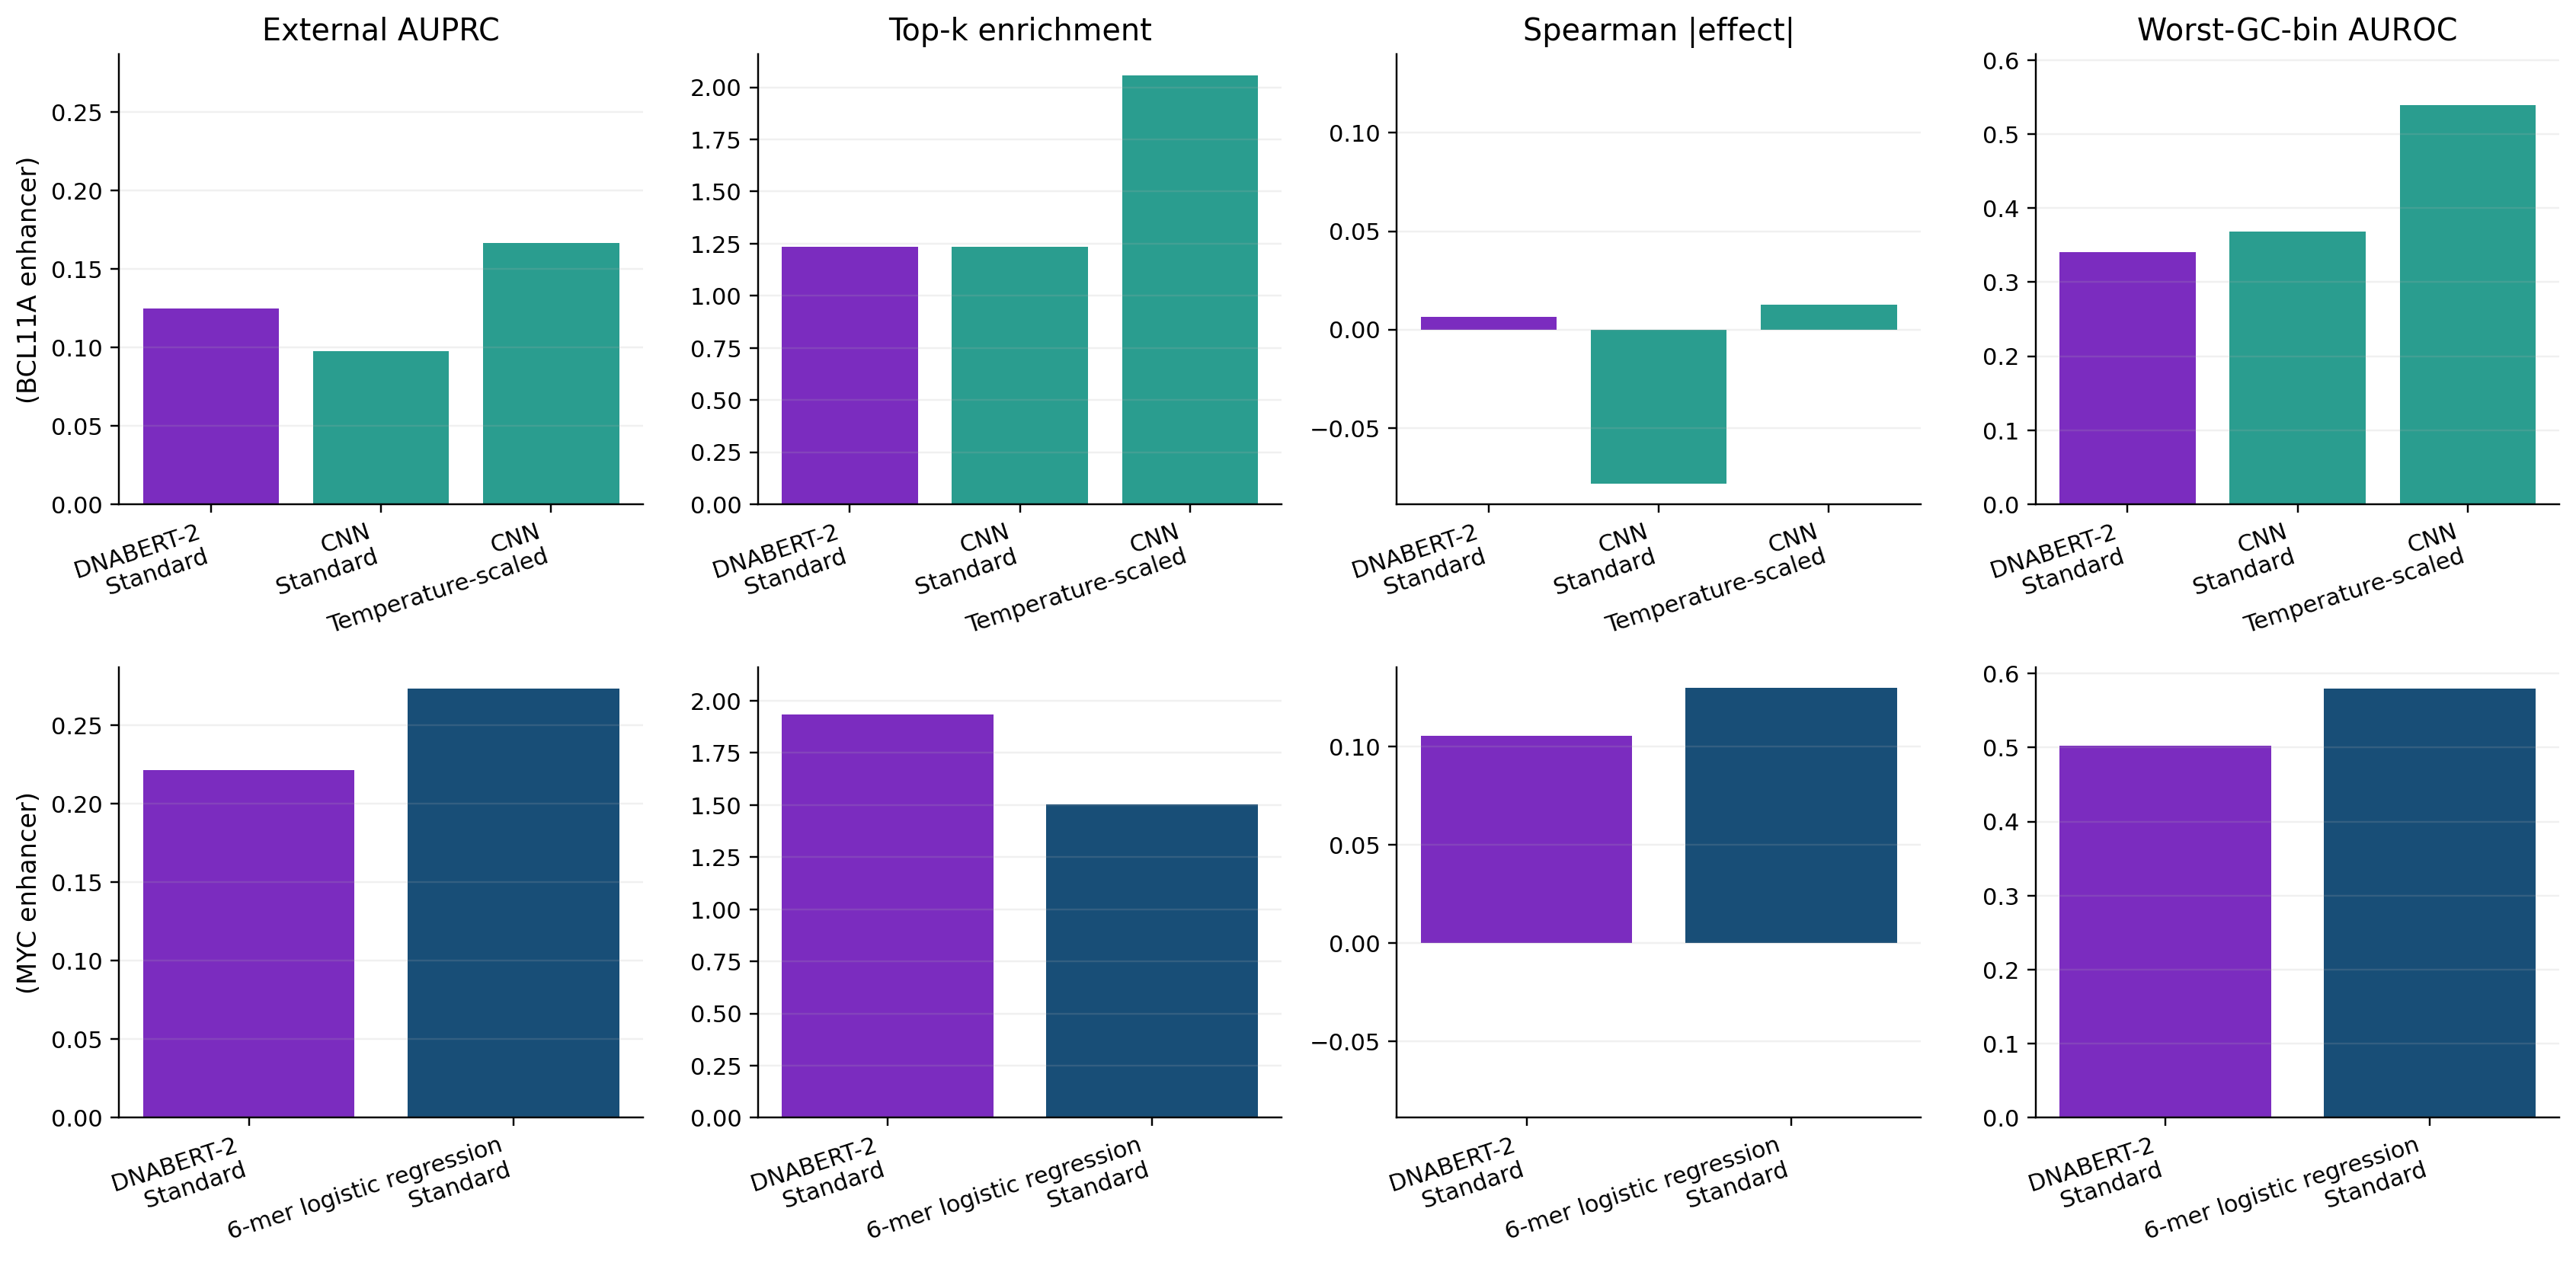
\includegraphics[width=\textwidth]{../figures/genomecf_biological_case_study.png}
  \caption{MPRA biological case studies. Case A shows that GenomeCF changes configuration choice on the BCL11A enhancer MPRA task by favoring a temperature-scaled CNN over the default CNN. Case B shows that GenomeCF changes model choice on the MYC enhancer MPRA task by favoring DNABERT-2 for top-ranked variant nomination even though the 6-mer baseline has stronger global AUROC and AUPRC.}
  \label{fig:case}
\end{figure*}

\begin{table*}[t]
  \centering
  \caption{MPRA case-study summary. The GenomeCF-aware recommendation changes configuration choice on BCL11A and model choice on MYC because the biologically useful external metrics differ from the held-out benchmark ranking.}
  \label{tab:case}
  \small
  \resizebox{\textwidth}{!}{\begin{tabular}{p{0.85cm}p{2.0cm}p{1.6cm}p{1.8cm}p{3.2cm}rrrrrr}
\toprule
Case & Task & Model & Config. & Decision role & Core ECE & External AUROC & External AUPRC & Top-k enrich. & Spearman & Worst-bin AUROC \\
\midrule
Case A & \shortstack[l]{MPRA BCL11A\\enhancer} & \shortstack[l]{CNN} & Standard & AUROC-only default configuration & 0.061 & 0.434 & 0.097 & 1.234 & -0.078 & 0.369 \\
Case A & \shortstack[l]{MPRA BCL11A\\enhancer} & \shortstack[l]{CNN} & Temperature-scaled & GenomeCF-aware configuration & 0.040 & 0.583 & 0.167 & 2.056 & 0.013 & 0.539 \\
Case A & \shortstack[l]{MPRA BCL11A\\enhancer} & \shortstack[l]{DNABERT-2} & Standard & Reference comparison & 0.029 & 0.540 & 0.125 & 1.234 & 0.007 & 0.340 \\
Case B & \shortstack[l]{MPRA MYC\\enhancer} & \shortstack[l]{DNABERT-2} & Standard & GenomeCF-aware variant-ranking choice & 0.029 & 0.580 & 0.221 & 1.934 & 0.105 & 0.503 \\
Case B & \shortstack[l]{MPRA MYC\\enhancer} & \shortstack[l]{6-mer logistic\\regression} & Standard & AUROC-only variant-ranking choice & 0.235 & 0.617 & 0.273 & 1.504 & 0.130 & 0.579 \\
\bottomrule
\end{tabular}
}
\end{table*}

\begin{table*}[t]
  \centering
  \caption{Controlled real-task motif probes. Small motif-minus-random effects indicate that the completed real-task predictions are not strongly explained by these simple known motif hits alone.}
  \label{tab:motif-main}
  \small
  \resizebox{\textwidth}{!}{\begin{tabular}{p{2.1cm}p{1.9cm}crrrrrr}
\toprule
Task & Model & n & Motif drop & GC-preserving & Random edit & Motif$-$random & Mono drop & Dinuc drop \\
\midrule
\shortstack[l]{Promoters} & \shortstack[l]{6-mer logistic\\regression} & 1000 & 0.015 & 0.011 & -0.005 & 0.019 & -0.003 & 0.058 \\
\shortstack[l]{Promoters} & \shortstack[l]{CNN} & 1000 & 0.010 & 0.006 & -0.000 & 0.010 & -0.002 & 0.046 \\
\shortstack[l]{Promoters} & \shortstack[l]{RC-aug CNN} & 1000 & 0.011 & 0.007 & 0.000 & 0.010 & -0.035 & 0.038 \\
\shortstack[l]{Promoters} & \shortstack[l]{DNABERT-2} & 1000 & 0.006 & 0.004 & 0.001 & 0.005 & -0.054 & 0.004 \\
\shortstack[l]{Promoters} & \shortstack[l]{Caduceus-Ph} & 1000 & 0.005 & 0.007 & -0.000 & 0.006 & -0.060 & 0.002 \\
\shortstack[l]{Enhancers\\(Cohn)} & \shortstack[l]{6-mer logistic\\regression} & 1000 & 0.009 & 0.012 & 0.003 & 0.006 & -0.080 & 0.138 \\
\shortstack[l]{Enhancers\\(Cohn)} & \shortstack[l]{CNN} & 1000 & -0.002 & 0.001 & 0.000 & -0.002 & 0.008 & 0.014 \\
\shortstack[l]{Enhancers\\(Cohn)} & \shortstack[l]{RC-aug CNN} & 1000 & -0.001 & 0.001 & -0.000 & -0.001 & 0.003 & 0.017 \\
\shortstack[l]{Enhancers\\(Cohn)} & \shortstack[l]{DNABERT-2} & 1000 & -0.000 & -0.002 & -0.001 & 0.001 & -0.049 & 0.023 \\
\shortstack[l]{Enhancers\\(Cohn)} & \shortstack[l]{Caduceus-Ph} & 1000 & -0.000 & 0.002 & -0.000 & 0.000 & -0.103 & -0.021 \\
\shortstack[l]{Enhancers\\(Ensembl)} & \shortstack[l]{6-mer logistic\\regression} & 1000 & 0.034 & 0.046 & 0.004 & 0.030 & 0.203 & 0.216 \\
\shortstack[l]{Enhancers\\(Ensembl)} & \shortstack[l]{CNN} & 1000 & 0.006 & 0.010 & 0.005 & 0.001 & 0.178 & 0.065 \\
\shortstack[l]{Enhancers\\(Ensembl)} & \shortstack[l]{RC-aug CNN} & 1000 & 0.004 & 0.009 & 0.005 & -0.001 & 0.320 & 0.127 \\
\shortstack[l]{Enhancers\\(Ensembl)} & \shortstack[l]{DNABERT-2} & 1000 & 0.012 & 0.019 & 0.002 & 0.010 & 0.043 & 0.009 \\
\shortstack[l]{Enhancers\\(Ensembl)} & \shortstack[l]{Caduceus-Ph} & 1000 & -0.000 & 0.003 & -0.000 & 0.000 & -0.032 & -0.009 \\
\bottomrule
\end{tabular}
}
\end{table*}

\subsection{GenomeCF-Synth isolates shortcut mechanisms under known ground truth}
GenomeCF-Synth is now a named sub-benchmark rather than a one-off diagnostic. It includes GC-correlated and GC-matched planted-motif tasks, a GC-conflict task, a two-motif grammar task and a motif-position conflict task. Figure~\ref{fig:synth} shows why these tasks are central to the resource.

In the original planted-motif pair, AUROC remains perfect in the GC-correlated setting even when motif sensitivity is essentially zero. For the 6-mer baseline, the GC-correlated motif-disruption drop is only 0.0004, whereas the same model becomes strongly motif-sensitive after GC matching, with mononucleotide-shuffle and motif-disruption drops 0.946 and 0.675. The conflict tasks sharpen that mechanism. In the GC-conflict task, DNABERT-2 and Caduceus-Ph both follow the shortcut 100\% of the time when the intended motif rule and GC shortcut disagree. In the motif-position conflict task, DNABERT-2 reaches AUROC 0.854 with rule-following rate 0.774, while the 6-mer model reaches AUROC 0.981 by following motif identity rather than position.

These tasks provide the cleanest proof that AUROC can reward shortcut learning and that different model families fail in different ways when rule and shortcut are separated. They also make GenomeCF-Synth reusable for future methods comparisons rather than tying it only to the current paper.

\begin{figure*}[t]
  \centering
  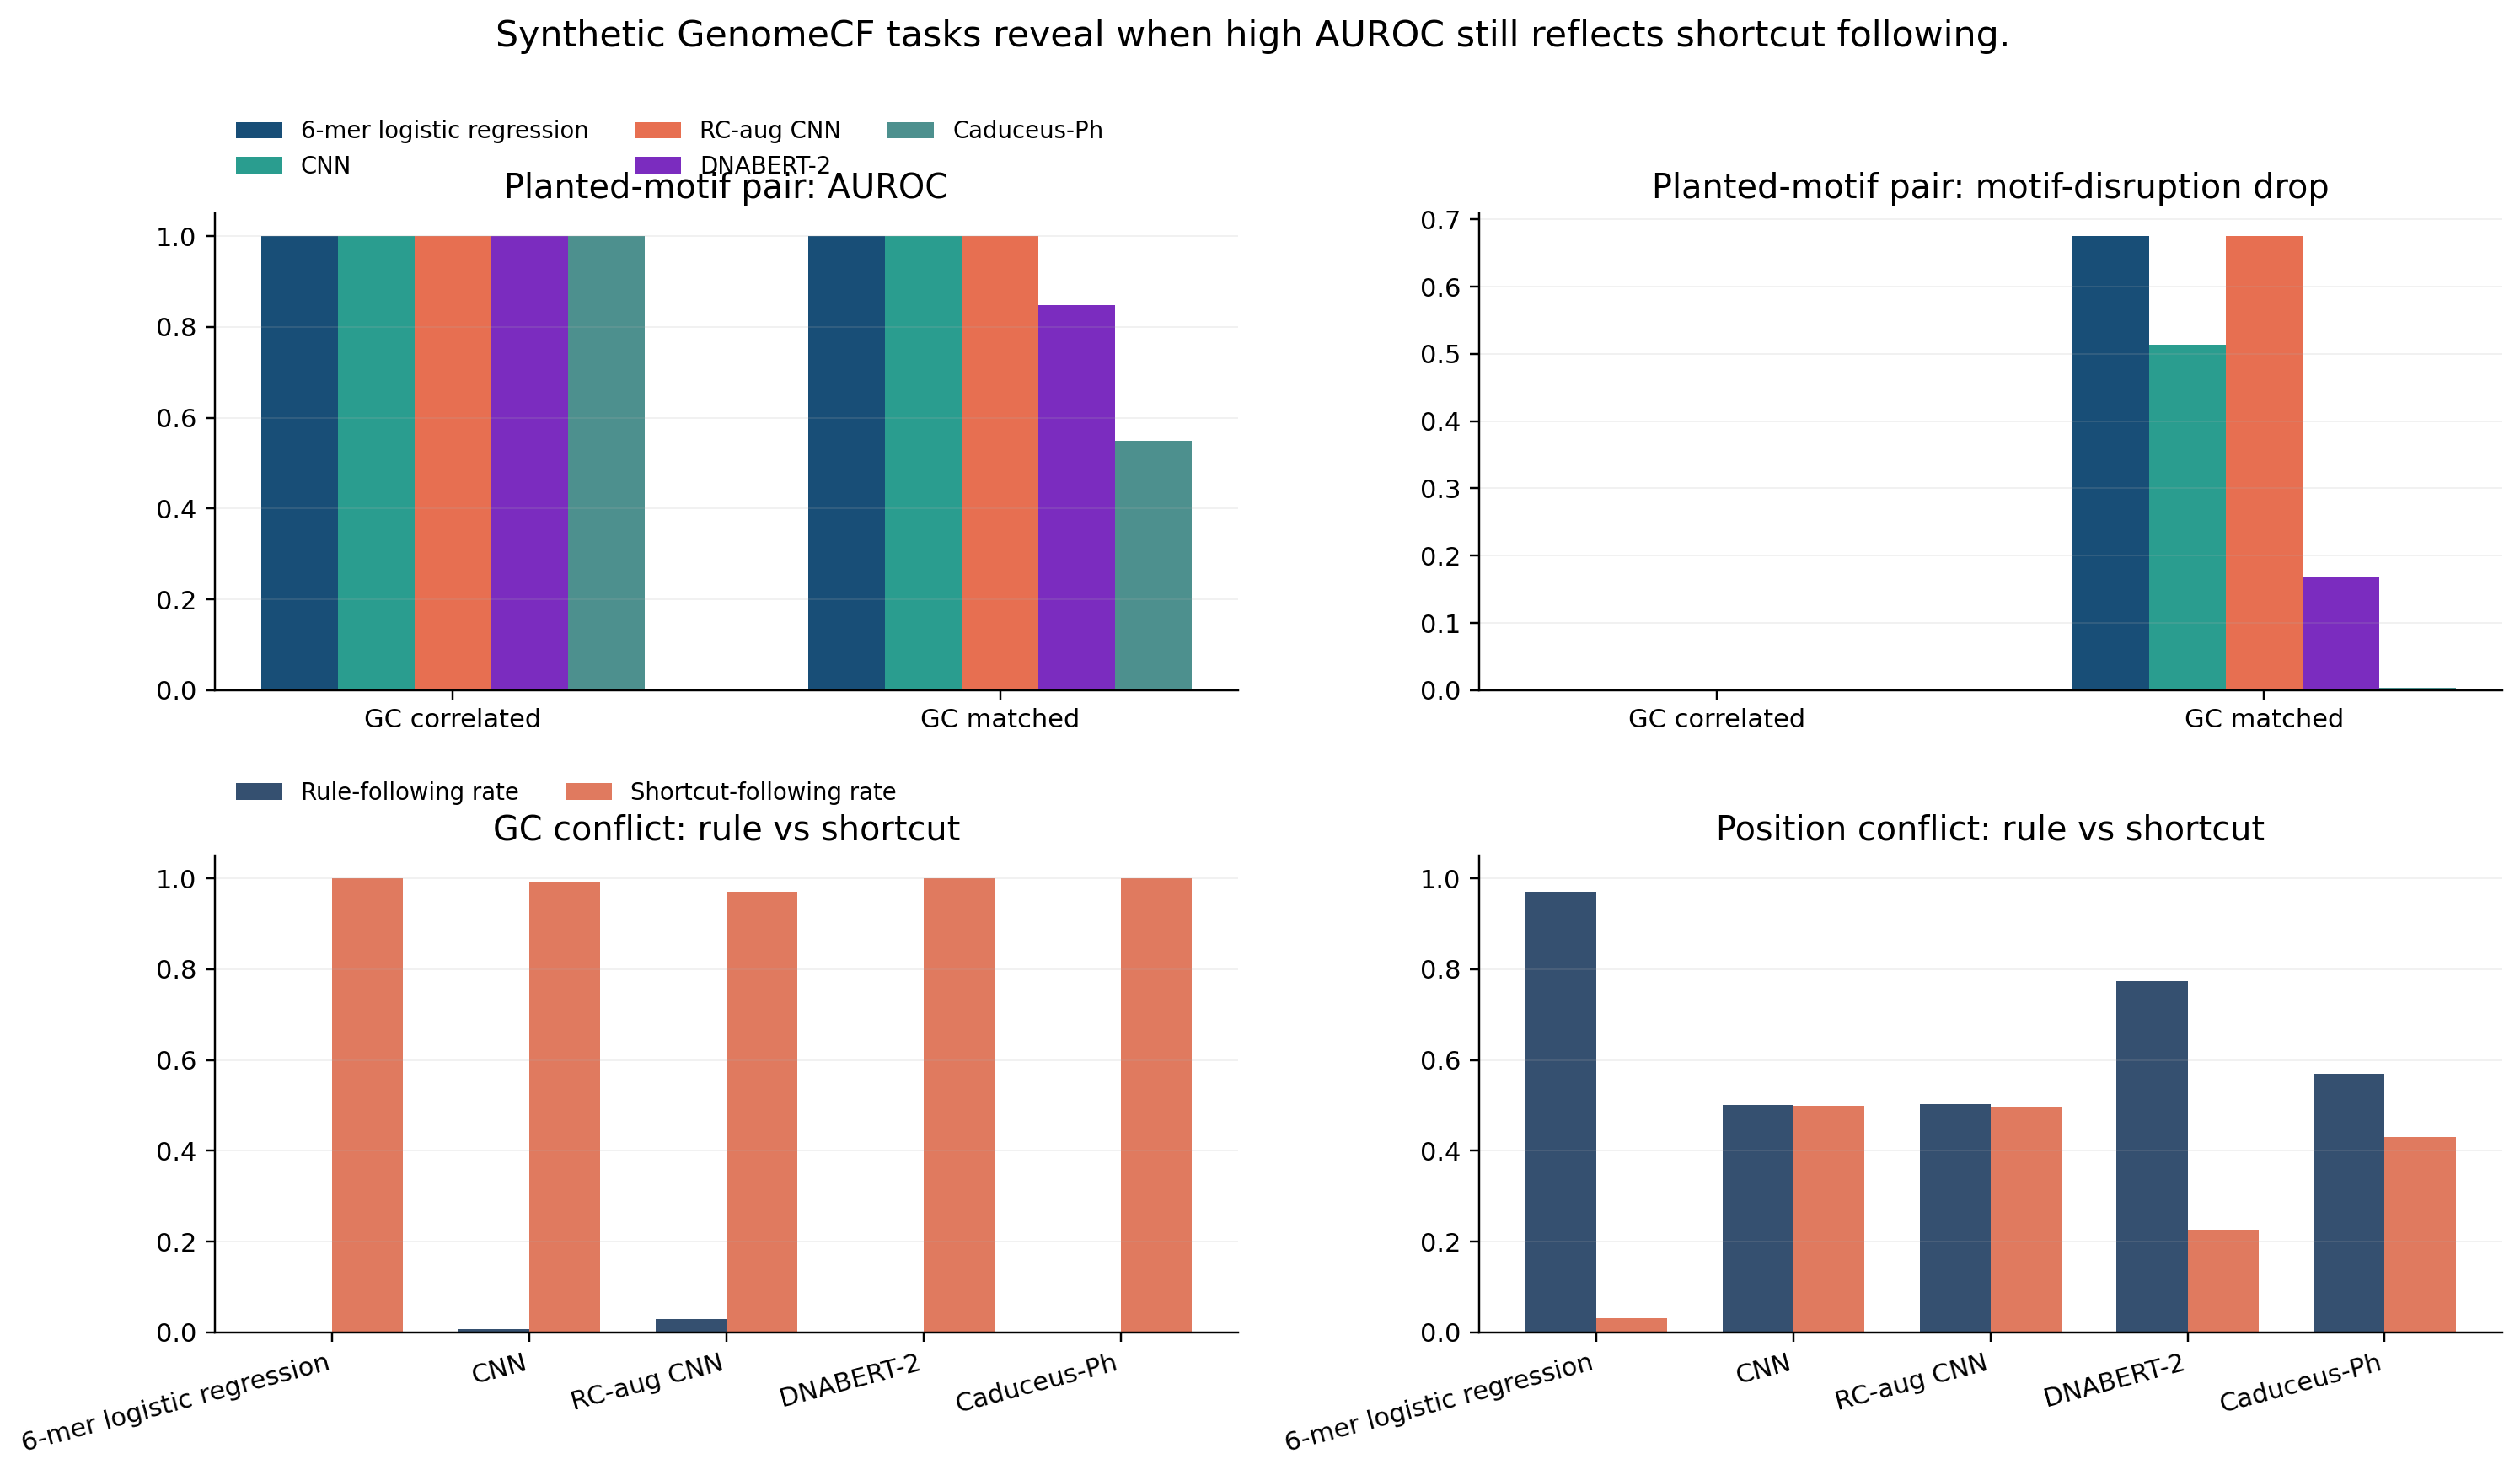
\includegraphics[width=\textwidth]{../figures/genomecf_synthetic_publication.png}
  \caption{GenomeCF-Synth. The top row revisits the planted-motif benchmark; the bottom row adds shortcut-conflict tasks that separate rule-following from shortcut-following behavior.}
  \label{fig:synth}
\end{figure*}

\subsection{GenomeCF supports a practical reporting standard and reusable software resource}
GenomeCF is intended to change how DNA sequence models are reported, not only how they are benchmarked. We therefore release the benchmark as a pip-installable package with a CLI, canonical registry, exported manifests, container setup, a quickstart path, a reporting checklist and a local website/leaderboard build. The reporting standard in Table~\ref{tab:checklist} is the minimal GenomeCF disclosure we recommend for future DNA sequence model papers. It includes held-out performance, perturbation response, calibration, confounder control, split robustness, synthetic conflict testing and registry traceability.

\begin{figure*}[t]
  \centering
  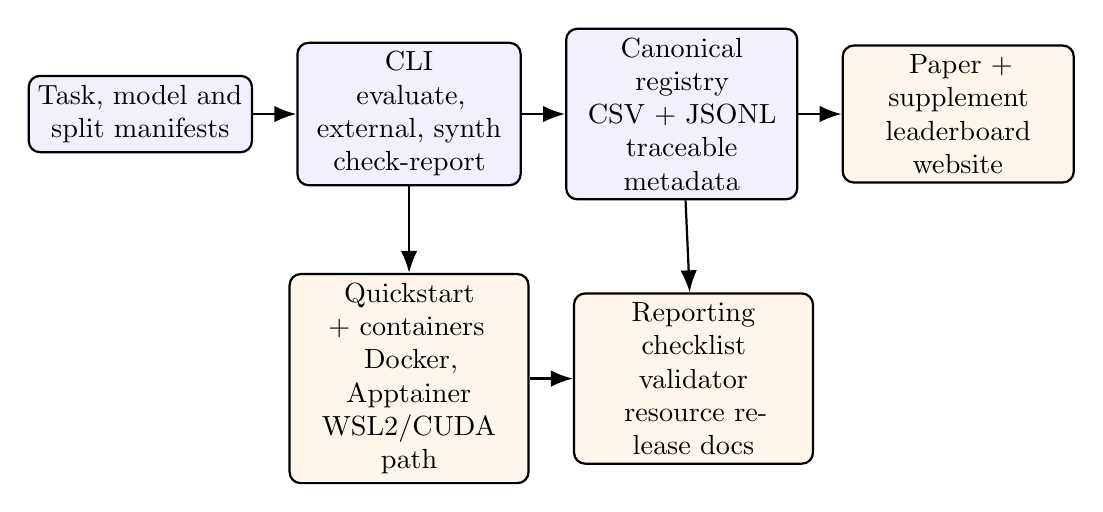
\begin{tikzpicture}[
    node distance=0.55cm and 0.55cm,
    box/.style={draw, rounded corners, thick, align=center, minimum height=0.95cm, fill=blue!6},
    outbox/.style={draw, rounded corners, thick, align=center, minimum height=0.95cm, fill=orange!8},
    arrow/.style={-{Latex[length=2.8mm]}, thick}
  ]
    \node[box, text width=2.6cm] (manifests) {Task, model and split manifests};
    \node[box, right=of manifests, text width=2.6cm] (cli) {CLI\\evaluate, external, synth\\check-report};
    \node[box, right=of cli, text width=2.7cm] (registry) {Canonical registry\\CSV + JSONL\\traceable metadata};
    \node[outbox, right=of registry, text width=2.7cm] (outputs) {Paper + supplement\\leaderboard\\website};
    \node[outbox, below=1.1cm of cli, text width=2.8cm] (quick) {Quickstart + containers\\Docker, Apptainer\\WSL2/CUDA path};
    \node[outbox, right=of quick, text width=2.8cm] (check) {Reporting checklist\\validator\\resource release docs};

    \draw[arrow] (manifests) -- (cli);
    \draw[arrow] (cli) -- (registry);
    \draw[arrow] (registry) -- (outputs);
    \draw[arrow] (cli) -- (quick);
    \draw[arrow] (registry) -- (check);
    \draw[arrow] (quick) -- (check);
  \end{tikzpicture}
  \caption{GenomeCF software and reporting workflow. The release includes manifests, CLI entry points, a canonical result registry, a quickstart path, container recipes, a reporting checklist and locally buildable website outputs.}
  \label{fig:resource}
\end{figure*}

\begin{table*}[t]
  \centering
  \caption{GenomeCF minimum reporting standard for DNA sequence model papers.}
  \label{tab:checklist}
  \small
  \begin{tabular}{p{5.4cm}p{8.8cm}}
    \toprule
    Category & Minimum items \\
    \midrule
    Held-out performance & AUROC, AUPRC, calibration on the original test set \\
    Counterfactual stability & Reverse-complement instability, reverse-complement flip rate, mononucleotide and dinucleotide shuffle response \\
    Calibration under stress & Original and perturbed ECE and Brier score \\
    Confounder control & Matched-negative evaluation and GC-bin worst-group AUROC \\
    Split robustness & Chromosome- or group-held-out evaluation \\
    Mechanism test & At least one GenomeCF-Synth shortcut-conflict task \\
    Reproducibility & Manifests, random seeds, leakage checks, registry-traceable outputs \\
    \bottomrule
  \end{tabular}
\end{table*}

\section{Discussion}
GenomeCF reframes DNA sequence model evaluation from pure prediction ranking toward reusable counterfactual validation. Across core regulatory tasks, external assay families, matched-negative controls, GC-stratified robustness, foundation-model adaptation and synthetic shortcut-conflict tests, the same pattern emerges: held-out AUROC is informative but insufficient. It does not reliably predict whether a model is stable to strand reversal, whether it is overconfident on shuffled or confounder-controlled sequences, or whether it will remain reliable on a related external assay.

The resource also sharpens how to interpret foundation models. DNABERT-2 tends to provide the strongest AUROC in the current release, while Caduceus-Ph often improves reverse-complement consistency. Neither model dominates every reliability axis. Matched-negative-trained heads and temperature scaling sometimes improve external or confounder-controlled behavior, but they do so selectively. GenomeCF is useful precisely because it exposes these tradeoffs rather than collapsing them into a single score.

Real-task mechanism analysis remains more nuanced than the synthetic benchmark. GenomeCF-Synth shows cleanly that the benchmark can detect motif-versus-shortcut behavior when the ground-truth rule is known. By contrast, the completed real regulatory tasks show only weak simple-motif sensitivity even after GC-preserving edits and random-edit controls. This is a meaningful negative result. It suggests that shortcut behavior in real DNA benchmarks is distributed across composition, context, annotation and background design rather than reducible to a small set of exact motif hits.

The remaining limitations are now scope expansions rather than missing core evidence. GenomeCF currently emphasizes short-context sequence classification plus compact experimentally grounded variant-effect assays rather than long-context sequence-to-function prediction or broader cell-type-specific regulatory panels. The external assay families are diverse enough to support the main resource claims, but larger community releases should add more MPRA, MAVE, cell-type transfer and causal variant datasets. Additional foundation models, deeper parameter-efficient tuning and richer long-context tasks remain natural next steps. But the central resource claims are already supported: GenomeCF provides a counterfactual validation standard, external biological validation, practical model-selection guidance and reproducible software for the genomics machine-learning community.

\section{Online Methods}
\paragraph{Benchmark tiers and data sources.}
The core benchmark contains four human Genomic Benchmarks tasks: \texttt{human\_nontata\_promoters}, \texttt{human\_enhancers\_cohn}, \texttt{human\_enhancers\_ensembl} and \texttt{human\_ocr\_ensembl}. Screening tasks remain separate from the main claims. External biological validation uses nine additional assay tasks: two human transcription-factor binding tasks and two human histone-mark tasks from the GUE/DNABERT-2 release, plus five human regulatory MPRA score sets from MaveDB derived from the saturation-mutagenesis study of disease-associated regulatory elements by \citet{kircher2019regulatory}. GenomeCF-Synth tasks are generated deterministically from versioned configuration files.

\paragraph{Models.}
The completed main-paper models are 6-mer logistic regression, CNN, RC-aug CNN, DNABERT-2 and Caduceus-Ph. Nucleotide Transformer v2 remains appendix-only diagnostic coverage because the current frozen mean-pooled protocol passed loader checks but did not pass internal benchmark validation strongly enough for main-paper use. DNABERT-2 and Caduceus-Ph use lower-data frozen-embedding subsets with the same logistic-regression head. Completed interventions include temperature scaling and matched-negative-trained frozen heads on the focal benchmark tasks, and completed Caduceus-Ph MPRA runs use the documented WSL2/Linux CUDA plus \texttt{mamba\_ssm} path with cached embeddings.

\paragraph{Perturbations and metrics.}
GenomeCF evaluates reverse complement, mononucleotide-preserving shuffle, dinucleotide-preserving shuffle, matched-negative evaluation and motif disruption. Main metrics include AUROC, AUPRC, ECE, Brier score, reverse-complement mean absolute probability change, reverse-complement flip rate, positive-probability drop under shuffles, matched-negative performance and GC-bin worst-group AUROC. The GenomeCF Shortcut Score is a summary diagnostic derived from within-task ranks of the raw reliability components and is reported only alongside the underlying metrics.

\paragraph{Statistical reporting.}
The external transfer analysis uses 82 model-configuration-task pairs across the completed external assays. We report Spearman or Pearson correlation coefficients with bootstrap confidence intervals, linear-model $R^2$ values with bootstrap intervals, family-stratified fits, leave-one-family-out validation summaries, and permutation comparisons between AUROC-only and GenomeCF-informed predictive models. Synthetic and motif-probe summaries are also stored in the release registry and supplementary tables.

\paragraph{Software and registry.}
All release-facing results are exported to a canonical registry in CSV and JSONL form. Publication tables and figures are generated from the release registry and derived summary files, not from manually copied values. The CLI exposes benchmark evaluation, external evaluation, synthetic evaluation, paper builds, appendix builds, report checking and quickstart reproduction.

\section{Data Availability}
GenomeCF task manifests, local preprocessing metadata, release tables and generated benchmark artifacts are included in the repository. External assay tasks distributed through GUE/DNABERT-2 retain their upstream licensing and data-availability terms. The MPRA variant-effect tasks are reconstructed from public MaveDB score sets and retain the upstream MaveDB licensing and citation requirements. Data paths and manifests are summarized in \texttt{docs/DATA\_AVAILABILITY.md}.

\section{Code Availability}
The GenomeCF software package, paper-generation scripts, benchmark registry, reporting checklist, container recipes and locally buildable website are included in the repository. The code-availability summary appears in \texttt{docs/CODE\_AVAILABILITY.md}.

\section{Benchmark Availability}
GenomeCF is released as a pip-installable package with a CLI, manifests, reproducibility scripts, a quickstart path, website assets and a reporting-checklist validator. The benchmark registry is stored in \texttt{results/release/benchmark\_registry.csv}. Practical release notes appear in \texttt{docs/NATURE\_METHODS\_RELEASE.md}.

\section{Model Availability}
Completed DNABERT-2 and Caduceus-Ph runs rely on public pretrained checkpoints, with Caduceus requiring the documented WSL2/Linux CUDA path. Model-specific notes appear in \texttt{docs/FOUNDATION\_MODELS.md} and \texttt{docs/CADUCEUS\_SETUP.md}.

\section{Environment Availability}
CPU-based smoke paths, paper builds and registry validation run in the default local environment. Larger foundation-model runs are documented for WSL2/Linux CUDA. Container recipes and environment files are provided for reproducible setup.

\section{Reproducibility Statement}
All main-paper figures and tables are generated from registry-backed results. The repository includes deterministic synthetic-task configs, smoke-test commands, benchmark manifests, environment notes, container files and registry validation scripts. The release-level checklist and reproduction commands are documented in \texttt{docs/REPRODUCIBILITY.md}.

\section{Competing Interests}
The author declares no competing interests.

\section{Author Contributions}
A.B. designed the benchmark, implemented the software and experiments, generated the figures and tables, and wrote the manuscript.

\section{Acknowledgements}
This project was developed as part of graduate work in machine learning and genomics at the University of California, Santa Cruz, and then extended into a reusable benchmark resource.

\section{Supplementary Information}
Supplementary tables, additional registry summaries, external-validation details, motif-probe details and release metadata are provided in the separate supplementary document.

\bibliographystyle{plainnat}
\bibliography{refs}

\end{document}

